\documentclass{article}
\usepackage[utf8]{inputenc}
\usepackage[margin=1.3in]{geometry}
\usepackage{amsmath}
\usepackage{amsthm}
\usepackage{amssymb}
\usepackage{appendix}
\usepackage{wasysym}
\usepackage{graphicx}
\usepackage{epstopdf}
\usepackage{wrapfig}
\usepackage{pdflscape}
\usepackage{bigints}
\usepackage{subfigure}
\usepackage{makecell}
\usepackage{diagbox}
\usepackage{multirow}
\usepackage{mcode}
\usepackage{hyperref}
\usepackage{mathtools}
\usepackage{float}
\usepackage{fancyhdr}

\pagestyle{fancy}
\fancyhf{}
\fancyhead[RE,LO]{Imperial College London}
\fancyhead[LE,RO]{Y. Chen, N. Desai, C. Goh, M. Sutharson, T.T. Trita}
\fancyfoot[CE,CO]{\thepage}

\setlength{\parskip}{0.3cm}
\setlength\parindent{0pt}

\makeatletter
\newcommand*{\rom}[1]{\expandafter\@slowromancap\romannumeral #1@}
\makeatother
\newcommand\myeq{\mathrel{\stackrel{\makebox[0pt]{\mbox{\normalfont\tiny set}}}{\equiv}}}
\newcommand\ddfrac[2]{\frac{\displaystyle #1}{\displaystyle #2}}
\newtheorem{theorem}{Theorem}[section]
\newtheorem{corollary}{Corollary}[theorem]
\newtheorem{lemma}[theorem]{Lemma}
\newtheorem{definition}{Definition}[section]
\newtheorem*{remark}{Remark}


\title{\textbf{The Distribution of the Extreme from a Normal Sample\\ M2R Project, Group 41, Prof. A.T. Walden}}
\author{Yifan Chen, Nishant Desai, Chang Goh, Maitanki Sutharson, Tudor Trita Trita}
\date{Imperial College London, 18th June 2018}

\begin{document}


\maketitle
\vspace{2cm}
\begin{center}
    \textbf{Abstract}
\end{center}

In this project, we look at the properties of maxima arising from normal random samples. We will find that asymptotically, there are only three types of distribution (Gumbel, Fr\'{e}chet and Weibull) that describe the data and these can be combined into one; the Generalised Extreme Value (GEV) distribution. We will begin by proving this result, known as the Fisher-Tippett Theorem, and then we present methods (MoM, MLE, PWM) for estimating the parameters of the Gumbel distribution and GEV distribution. We then look at Quantile-Quantile (QQ) plots and Bootstrapping techniques, which find the model with the best fit.

The project then focuses on analysing earthquake data from Greece to be able to derive statistical properties and make future predictions.  We do this by fitting a Gumbel distribution and GEV distribution to the Greece earthquake data, and estimating parameters for each model using the methods above. We then use QQ plots and Bootstrap Confidence Intervals to find the model that fits the Greek earthquake data the most. Finally, we look at return periods which will give predictions as to when to expect the next earthquake of a given magnitude.

\newpage
\tableofcontents
\newpage
%%%%%%%%%%%%%%%%%%%%%%%%%%%%%%%%%%% Submitted by Maitanki 12/06/2018

\section{Introduction}

Modelling extreme events has been crucial in seismography, oceanography and insurance. One of the first applications of Extreme Value distributions was modelling flood flows, made by Fuller in 1914. In 1920, Griffith applied extreme value theory to the behaviour of flow and fracture in solids. In the 1940s, Gumbel played a crucial role introducing more exciting applications of extrema, including radioactive emissions and human lifespans. (Kotz \& Nadarajah, 2000) 

The maxima are taken from a large sample of independent and identically distributed random variables. As the sample size goes to infinity, the behaviour of the maxima is described by the three Extreme Value distributions - Type 1 (Gumbel), Type 2 (Fr\'echet) and Type 3 (Weibull), which can be written as a unified distribution, the Generalised Extreme Value (GEV) distribution.

Gumbel, Fr\'echet and Weibull consist of 2 parameters, $\mu$ and $\sigma$, with $k=0$, $k>0$ and $k<0$ for Gumbel, Fr\'echet and Weibull respectively. GEV distribution has 3 parameters: $\mu$, $\sigma$ and $k$. (Coles, 2001)

Extreme Value distributions have several applications in the environmental science. The GEV distribution has been used for flood frequency analysis in the UK to model daily or annual maxima of natural occurrences, for example rainfall, sea levels and river lengths.
%just added 69+71 (check)
Gumbel distribution has been used heavily in hydrology for modelling extreme events, engineering and annual flood flows in 1958. Fr\'echet distribution has had many applications in finance including modelling market returns, which generally have heavy tails. Weibull distribution initially was developed to observe minima in material analysis. (Alves \& Neves, 2008) The GEV distribution is usually used to model the extrema of long finite sequences of random variables.

In 1990, de Haan estimated the parameters, $\psi$ in the distribution based on the high-tide water levels at Hoek van Holland, the Dutch Station during 1887 until 1984.
\begin{equation*}
    G_\psi(x) = \begin{cases}
    \exp(-(1+\psi x)^{1/\psi}), & \text{$1 + \psi x > 0$},\\
    \exp(-(\exp(-x))), & \text{$\psi=0$}.
  \end{cases}
\end{equation*}

If $\psi = 0$, the water levels follow a Gumbel distribution (under GEV with $\psi=0$) with $\mu=0$ and $\sigma=1$, and if $1+ \psi x >0$, it is a GEV distribution (Fr\'echet and Weibull) with $\mu=0$ and $\sigma=1$. (Kotz \& Nadarajah, 2000)

In 1995, Robinson and Tawn used the GEV distribution to see whether an athlete's record is better than the ultimate performance predicted by the data. The performance of Wang Junxia, a Chinese 3000m flat track athlete in Beijing national championship ran her personal best of 486.11 seconds (1993). Her time was 6.08 seconds faster than the day before, and 10.43 seconds faster than her previous record, hence there was suspicion the record was drug assisted.

Annual minima for the women's 3000m race from 1972-1992 with Junxia's time in 1993 was considered in order to determine whether her performance was drug-enhanced. A confidence interval with the GEV distribution was constructed to find the minimum time possible time- this was insufficient to reach a conclusion. Therefore the five best annual times for 3000m is included, meaning Wang's time is within the 90\% confidence interval (430.1, 493.8). Alongside this, incorporating relative performances in 1500m events (478.4, 495.0) and Olympic and World championship years (486.3, 497.0), Wang's time is within the 90\% confidence interval. Therefore, Robinson and Tawn concluded that there is no legal case that can say Wang's performance in 1993 was drug-enhanced; her time is within the 90\% confidence interval for the ultimate time. (Smith, 2009)

The above applications are based on the data of the maxima will fit an Extreme Value distribution. In order to find this distribution, the parameters (location, scale, shape) need to be estimated for Gumbel distribution and GEV distribution. There are three main methods of parameter estimation, Method of Moments, Maximum Likelihood Estimation and Probability Weighted Moments. It is important to compare these methods of parameter estimation as Figure 1 highlights that different sets of parameters give very different PDFs.  

These estimation methods will be discussed and compared in detail for Extreme Value distributions, and put into practice the worked example. After estimating the parameters for Gumbel distribution and GEV distribution, the goodness of fit needs to be tested with Quantile-Quantile plots (QQ plots) and Bootstrap Confidence Intervals.

Using these results, the return value is calculated, which estimates the frequency of extreme quantiles occurring with a certain level. This will be useful in risk management, as information about the likelihood of rare events can be gathered. (National Aeronautics and Space Administration, 2018)

In the second part of the report, the worked example will analyse earthquake data in Greece
from 1901-2017. The data will be modelled as Extreme Value distributions, either Gumbel distribution
or GEV distribution, with its parameters estimated by Method of Moments, Maximum
Likelihood Estimation and Probability Weighted Moments. The goodness of fit for each of the
models will tested by QQ plots and Parametric Bootstrap to find the best model. A conclusion will then be made taking the return level into account.

\vspace{1cm}
\begin{figure}[h]
\begin{center}
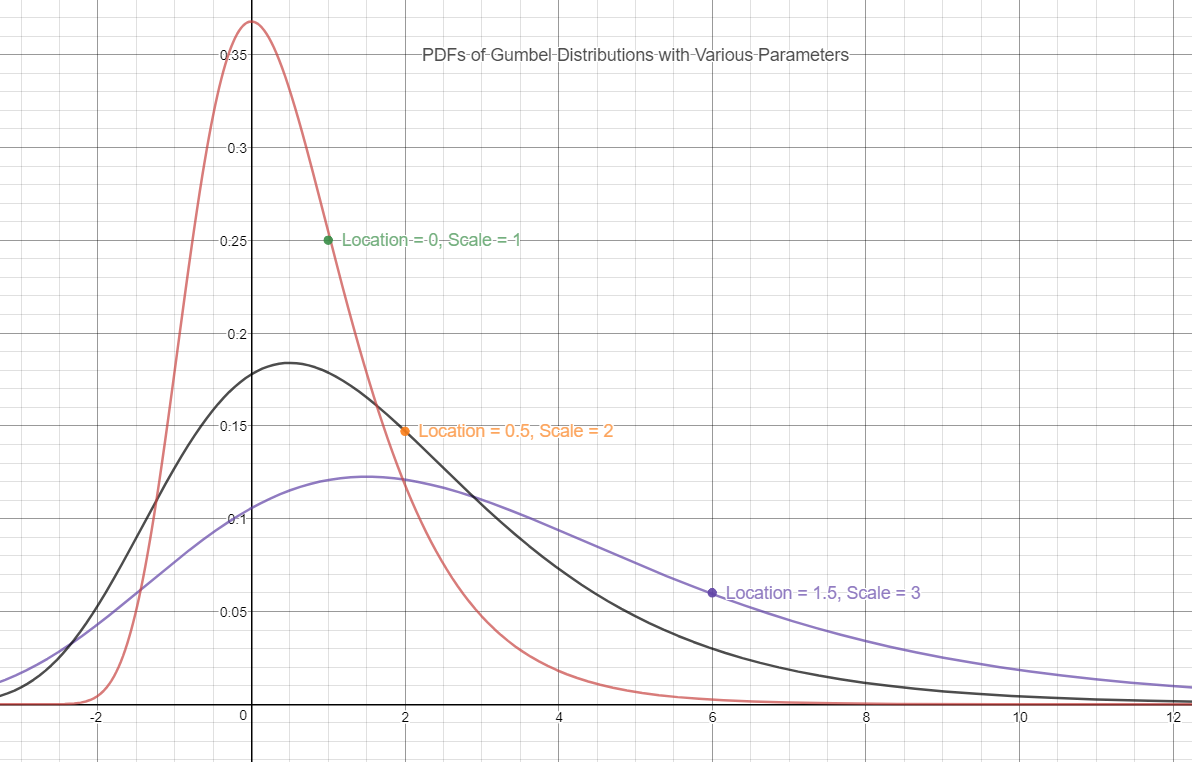
\includegraphics[width = 13.5cm, height = 9cm]{GumbelPDFSection1.png}
\caption{PDFs of Gumbel Distributions with Various Parameters}
\end{center}
\end{figure}



\newpage
%%%%%%%%%%%%%%%%%%%%%%%%%%%%%%%%%%%%%%%%%%

\section{Extreme Value Distributions}
\subsection{Model Formulation}
%Billy message 10/06/2018 implemented 22:00

We consider a model focused on the statistical behaviour of
$M_n=\max{\{X_1,X_2,\ldots,X_n\}},$ 
where  $X_1,X_2,\ldots,X_n$ is a sequence of independent random variables having a common
distribution function $F$.

The $X_i$s are the measurements on a regular time period and $M_n$ is the maximum value over the n observations in the entire time period.

As the $X_i$ are i.i.d., we know that
$$\Pr\{M_n\leqslant x\}=\Pr\{X_1\leqslant x,\ldots,X_n\leqslant x\}=\Pr\{X_1\leqslant x\}*\ldots*\Pr\{X_n\leqslant x\}=\{F\{x\}\}^{n}.$$

However, as the distribution function of $F$ is unknown, $\Pr\{M_n \leqslant x\}=\{F\{x\}\}^{n}$ is not useful yet at this point.

We choose to accept that $F$ is unknown and look at the families of models of $F^n$ instead. We start by considering the behaviour of $F^n$ as n tends to infinity. For any $X<X_+$, where $X_+$ is the upper end point of $F$, ($x_+$ is the smallest value of x such that $F(x)=1$, $F^{n} (x)\to 0$ as $n \to \infty$ and so distribution of $M_n$ degenerates to a point mass on $x_+$. This difficulty is avoided by allowing a linear renormalisation of the variable $M_n$: 

$$M_n^*=\frac{{M_n}-{b_n}}{a_n}$$ 
with appropriate choices of the sequences of constants $\{a_n>0\}$ and $\{b_n\}$ which stabilise the location and scale of $M_n^*$ as n increases respectively. (Page 46, Coles, 2001).

If there exist sequences of constants $\{a_n\}$ and $\{b_n\}$ such that $$\Pr\left(\frac{{M_n}-{b_n}}{a_n} \leqslant x\right) \to G(x), \quad \text{as} \quad n\to \infty,$$
where $G$ is a non-degenerate distribution function, then $G$ belongs to one of the following families:
\begin{align}
\textbf{Type \rom{1}}&: G(x) = \exp\left(-\exp\left(-\frac{x-\mu}{\sigma}\right)\right), \quad \forall x \in \mathbb{R}.\label{maingumble}\\
\textbf{Type \rom{2}}&: G(x) = \exp\left(-\left({\frac{x-\mu}{\sigma}}\right)^{-k}\right),\text{ if } x\geq \mu, \text{ and } G(x) = 0 \text{ otherwise.}\label{mainfrechet}\\
\textbf{Type \rom{3}}&: G(x) = \exp\left(-\left(-\frac{x-\mu}{\sigma}\right)^{k}\right),\text{ if } x\leq \mu, \text{ and } G(x)=1\text{ otherwise.}\label{mainweibull}
\end{align}
for parameters $\sigma>0$, $\mu \in \mathbb{R}$ and in the case of types \rom{2} and \rom{3}, $k>0$. (Page 46, Coles, 2001)

The three families are the extreme value distributions known as \textbf{Gumbel, Fr\'{e}chet and Weibull} respectively with location and scale parameters $\mu$, $\sigma$ resp. and $k$ is the shape parameter.

\subsection{The GEV Distribution}
It is in general difficult to know which distribution to adopt and subsequently this may produce errors in the estimates of the parameters of the distributions. Furthermore, once the choice is made, subsequent inference presume the choice to be correct and not allowing for uncertainty in such a choice would make errors substantial. (Page 47, Coles, 2001)

We therefore generalise the three families and combine them into a single family of models CDF of the form

\begin{equation}
G(z)=
\begin{dcases}
\exp\left(-\left(1+k\ \frac{x-\mu}{\sigma}\right)^{-1/k}\right), & \text{if } k \neq 0,\\
\exp\left(-\exp\left(-\frac{x-\mu}{\sigma}\right)\right), & \text{if } k = 0,\label{maingev}
\end{dcases}
\end{equation}
defined on set $\{x:1+k((z-\mu)/\sigma) > 0\}$ for $-\infty < \mu < \infty,\ \sigma > 0,\  -\infty < k < \infty$. (Page 47,48, Coles, 2001)

This is called the \textbf{Generalised Extreme Value} (GEV) family of distributions. Here $\mu$ is the location parameter, $\sigma$ is the scale parameter and $k$ is the shape parameter. Particularly, if when $k>0$ resp. $k<0$, then a Fr\'echet resp. Weibull family occurs.

We now consider the case when $k \to 0$ and we find that 
$$G(x) \to \exp\left(-\exp\left(-\frac{x-\mu}{\sigma}\right)\right),$$ 
which is exactly the same as a Gumbel family.

Generally, we say $G$ is a member of the GEV family if there exist sequences of constants $a_n>0$ and $b_n$ such that 
$$\Pr\left(\frac{{M_n}-{b_n}}{a_n} \leqslant x\right) \to G(x), \quad \text{as} \quad n\to \infty,$$
and equivalently, for large enough $n, \ \Pr(M_n \leqslant x) \approx G((x-b_n)/a_n)=G^{*}(x)$ where $G^{*}(x)$ is another member of the GEV family. (Page 48, Coles, 2001)

\subsection{Return Levels and Return Periods}
Additionally, we consider $z_p$, the return level associated with the return period $1/p$, the level $z_p$ is precisely exceeded by the annual maximum in any particular year with probability p, where 
$$ z_p=
\begin{cases} 
\mu-(\sigma/k)[1-(-\log(1-p))^{-k}], & k\ne 0,\\
\mu -\sigma \log\{-\log(1-p)\},  &k=0.\\
\end{cases}
$$

It is said in (Coles, 2001) that  ‘‘since quantiles enable probability models to be expressed on the scale of data, the relationship of the GEV model to its parameters is most easily interpreted in terms of the quantile expressions. In particular, defining $y_p=-\log(1-p)$, such that
$$z_p=
\begin{cases} \mu-(\sigma/k)[1-{y_p}^{-k}], & k\ne 0,\\
\mu-\sigma \log y_p, & k=0.
\end{cases}
$$

It follows that if $z_p$ is plotted against $y_p$ on a logarithmic scale, the plot is linear in the case $k=0$. If $k<0$, the plot is convex with asymptotic limit as $p \to 0$ at $(\mu-\sigma)/k$. If $k>0$ the plot is concave and has no finite bound and this graph is a return level plot.''

%%%%%%%%%%%%%%%

We illustrate this by looking at Figure \ref{fig:sec2returnplot} above.

We generate 100 random samples and fit them into a model of Gumbel and GEV and then we create the plot of return level against return period. For the sake of simplicity, assume that the return level represents magnitude and the return period is measured in years in the graph above. We can therefore make predictions; for the GEV model, an event of magnitude 10 will on average occur every 180 years, and for the Gumbel model, an event of magnitude 10 will on average occur every 40 years. 

In particular, one can find out the specific return period T of a particular level by solving the equation
$$T=\frac{1}{1-G(Z_p)}.$$

For example, if we want the return period for an event of magnitude 5, it would occur in 2.0163 years for GEV and 1.7462 for Gumbel.

\begin{figure}
    \centering
    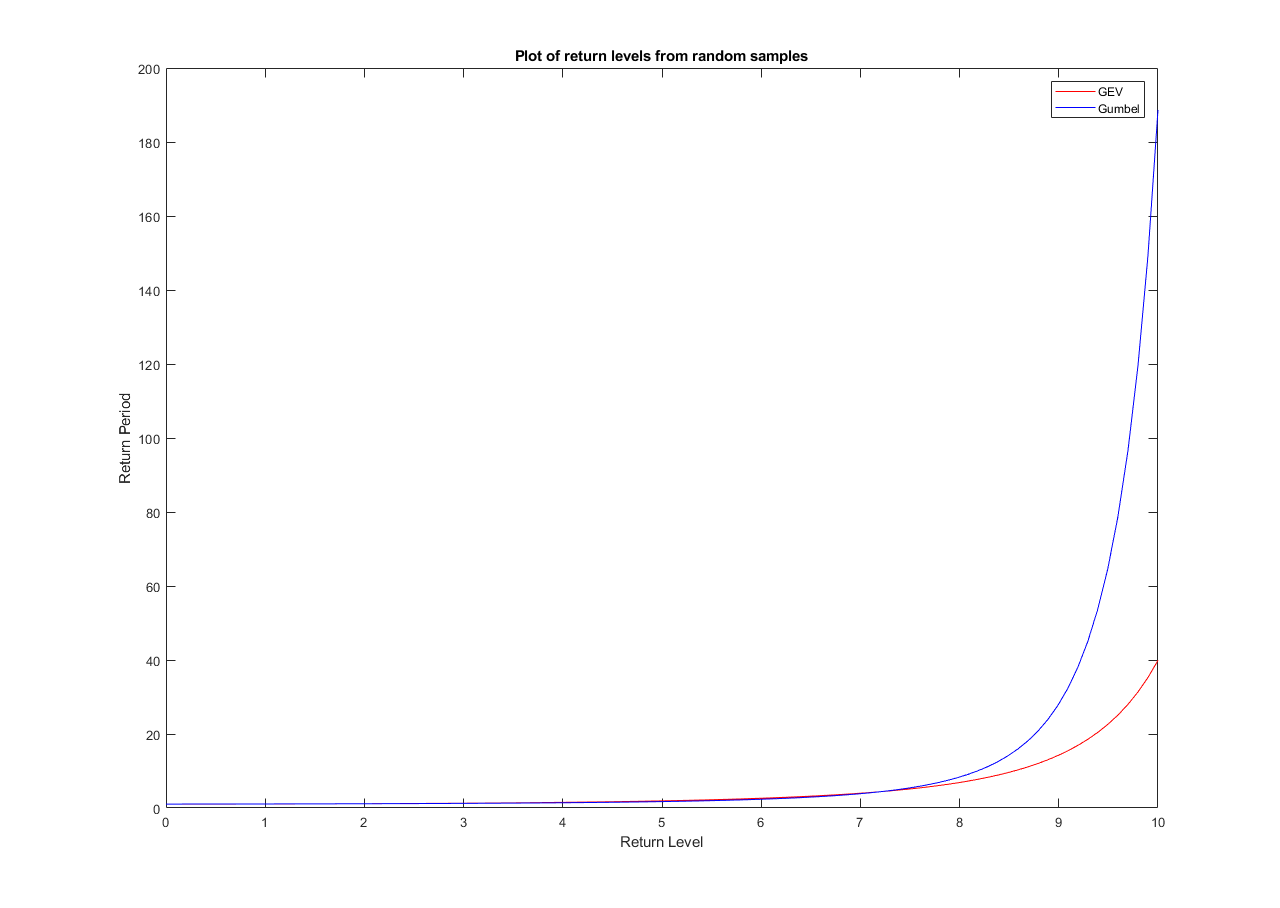
\includegraphics[width = 15cm, height = 9cm]{theoryreturnplot.png}
    \vspace{-10mm}
    \caption{Plot of Return Levels from Random Samples}
    \label{fig:sec2returnplot}
\end{figure}

%%%%%%%%%%%%%%%%%%%%%%%%%%%%%%%%%%%
\newpage
%%%%%%%%%%%%%%%%%%%%%%%%%%%%%%%%%%%
\section{Asymptotic Properties}

% References, (Nadarajah, 2018), (Sun, 2018)


The goal of this section is to formalise the claims of Section 2.1. 

We begin with some definitions:

\begin{definition}[Type of Distribution]
Let $X$ and $Y$ be two random variables with distributions $\mu$ and $\nu$ respectively. We say that $\mu$ and $\nu$ are of the same \textbf{type} if there exists $a > 0$ and $b \in \mathbb{R}$ such that $aX + b$ has the same distribution as $Y$.
\end{definition}

\begin{definition}[Max-Stable Distributions, (Sun, 2018)]
A non-degenerate probability distribution $\mu$ on $\mathbb{R}$ is called max-stable if for a sequence of i.i.d random variables $(X_{i})_{i\in\mathbb{N}}$ with distribution $\mu$ and for each $n\in\mathbb{N}$, there exists $a_n > 0$ and $b_n \in\mathbb{R}$ such that $(M_{n} - b_{n})/a_{n}$ also has distribution $\mu$.

Equivalently, $\mu$ is max-stable if its CDF $F(x):= \mu(-\infty,x]$ satisfies: for each $n\in\mathbb{N}$, there exists $a_{n} > 0$ and $b_n \in \mathbb{R}$ such that:
\[F^{n}(a_n x + b_n) = F(x), \forall x \in \mathbb{R}. \]
\end{definition}

\begin{remark}
Note that $M_n := \max\limits_{1 \leq i \leq n} X_i.$
\end{remark}

The following lemma is useful in proving the main result that follows.

\begin{lemma}
If $G$ is max-stable, then there exist real-valued functions $a(s) > 0$, and $b(s)$ defined for $s>0$, such that:
\[ G^{n}(a(s)x + b(s)) = G(x).\]
\end{lemma}
%%%%%%%%%%%%%%%%%%%%%%%%%%%%%%%%%%%%%%%%%%%%%%%%%%%%%%%%%%%%%%%%%%%%%%%%
%%%%%%%%%%%%%%%%%%%%%%%%%%%%%%%%%%%%%%%%%%%%%%%%%%%%%%%%%%%%%%%%%%%%%%%

The main theorem of this section, the Extremal Types Theorem, also known as the Fisher-Tippett-Gnedenko Theorem:

\begin{theorem}[Extremal Types Theorem]
Let $X_1,\ldots,X_n$ be i.i.d. with CDF F and let $X_{(n)} = \max\limits_{1 \leq i \leq n} X_{(i)}$. If there exist constants $a_n > 0 $ and $b_n$ and a non-degenerate distribution function G such that
$$\Pr \left( \frac{X_{(n)}-b_n}{a_n} \leq x \right) \xrightarrow{D}G(x), $$
then G must be of the same type as one of the three extreme value distributions (Gumbel, Fr\'echet, Weibull).

Conversely, any distribution function of the same type as one of these extreme value
classes can appear as such a limit. (Nadarajah, 2018a)
\end{theorem}

\begin{proof}
\textit{This proof very closely follows} (Nadarajah, 2018a). To prove the theory, it suffices to check that the set of max-stable distribution functions is the same as the set of distribution functions of the same type as the Gumbel, Fr\'echet and Weibull distributions.

Step 1: Check that the Gumbel, Fr\'echet and Weibull distributions are max-stable.

For Gumbel, if $a_n=1, b_n=\log{n}$, then
\begin{align*}
    G^{n}(a_nx+b_n) &= \exp(-n\exp-(a_nx+b_n)),\\
                    &= G(x).
\end{align*}

For Fr\'echet, if $a_n = n^{1/\alpha}, b_n = 0$, then:
\begin{align*}
    G^{n}(a_nx+b_n) &= \exp(-n(a_nx+b_n)^{-\alpha}), \text{ if } x > 0, \text{ and zero otherwise,}\\
                    &= G(x).
\end{align*}

For Weibull, if $a_n =n^{-1/\alpha},b_n=0$, then:
\begin{align*}
    G^{n}(a_nx+b_n) &= \exp(-n(-a_nx-b_n)^{\alpha}), \text{ if } x < 0, \text{ and one otherwise,}\\
                    &= G(x).
\end{align*}

Thus we have checked that $G^{n}(a_n x+ b_n) = G(x)$ in all three cases, thus they are max-stable.

Step 2: Now suppose G is max-stable, then by \textbf{Lemma 3.1},
$$G^s(a(s)x+b(s))=G(x).$$

Taking logs, for $0<G(x)<1$,
$$-\log(\log(G(a(s)x+b(s))))-\log s = \log(-\log G(x)).$$

The max-stability property with $n = 2$ implies that $G^2(ax+b) = G(x)$ for some $a>0$ and $b\in\mathbb{R},$ so that G does not jump at $x_{-}=\sup\{x:G(x)=0\}$ or $x_{+} = \inf\{x:G(x)=1\}$ if these are finite. (Nadarajah, 2018a)

Thus, the non-decreasing function $\phi(x)=-\log(-\log G(x))$ is such that
$$ \lim_{x \to x_-} \phi(x) = -\infty,\qquad \lim_{x \to x_+} \phi(x) = +\infty. $$

Therefore, $\phi$ has an inverse function $U(y)=\inf\{x\in\mathbb{R}:\phi(x)\geq y\}, \forall y\in\mathbb{R}.$ Now, $\phi(a(s)x+b(s))-\log s = \phi(x)$, it follows that:
\begin{align*}
    U(y) &= \inf\{x:\phi a(a(s)x+b(s))-\log s \geq y\},\\
         &= \frac{1}{a(s)}[\inf\{x^{\prime}:\phi(x^{\prime})\geq y + \log s\} - b(s)],\\
         &= \frac{U(y+\log s) -b(s)}{a(s)}.
\end{align*}

Subtracting for $y=0$,
$$\frac{U(y+\log s)-U(\log s)}{a(s)} = U(y) - U(0),$$

Write $z=\log s, \quad \tilde{\eta}(z)=a(e^{z}),\quad \Tilde{U}(y)=U(y)-U(0).$
\begin{equation}
    \Tilde{U}(y+z)-\Tilde{U}(z)=\Tilde{U}(y)\tilde{\eta}(z),\quad \forall y,z\in\mathbb{R}.\label{proof1}
\end{equation}
Interchanging y and z and subtracting,
\begin{equation}
    \Tilde{U}(y)(1-\tilde{\eta}(z))=\Tilde{U}(z)(1-\tilde{\eta}(y)).\label{proof2}
\end{equation}

\textbf{Case 1:} $\tilde{\eta}(z_0)\neq 1$ for some $z_0 > 0.$\vspace{0.5cm}

Then $\tilde{\eta}(z)\neq1, \forall z > 0,$ because otherwise $\exists z>0,$ s.t. $\tilde{U}(z) = 0.$ But then $\tilde{U}(y+z) =\tilde{U}(y),\forall y $ by (\ref{proof1}), so $U(y+z)=U(y) \ \forall y\in\mathbb{R}.$ This is a contradiction.

Fixing $z>0$, writing $c=\tilde{U}(z)/(1-\tilde{\eta}(z))$ and noting from (\ref{proof2}) that this is constant, we have from (\ref{proof1}) that
$$c(1-\tilde{\eta}(y+z))-c(1-\tilde{\eta}(z))=c(1-\tilde{\eta}(y))\tilde{\eta}(z),$$
such that
$$\tilde{\eta}(y+z)=\tilde{\eta}(y)\tilde{\eta}(z),\quad \forall y \in \mathbb{R}.$$

But $\tilde{\eta}$ is monotone, since $\tilde{U}(y)=c(1-\tilde{\eta}(y))$ from (\ref{proof2}), and the only non-zero solutions that are monotone and not identically equal to 1 are $\tilde{\eta}(y)=\exp(\rho y)$ for some $\rho \neq 0.$ But then
$$\phi^{-1}(y)=U(y)=\zeta + c(1-e^{\rho y}),$$
where $\zeta = U(0)$. Since $\phi^{-1}$ is non-decreasing, we must have that $c<0$ if $\rho>0$ and $c>0$ if $\rho<0$, so in fact $\phi^{-1}$ is continuous and strictly increasing.

Hence $$x=\phi^{-1}(\phi(x))=\zeta + c\left(1-e^{\rho\phi(x)}\right)=\zeta + c(1-(-\log G(x))^{-\rho}),$$
so $$G(x) = \exp\left(-\left(1-\frac{x-\zeta}{c}\right)^{-\frac{1}{\rho}}\right),\quad \text{for } 0<G(x)<1.$$

From the continuity of G at any finite endpoints, we see that G is of Type \rom{2}, with $\alpha=1/\rho$, if $\rho>0$, and of Type \rom{3}, with $\alpha = -1/\rho$, if $\rho <0.$\vspace{0.5cm}

\textbf{Case 2:} $\tilde{\eta}(z)=1, \ \forall z> 0.$

But then, from (\ref{proof1}), $\tilde{U}(y+z)=\tilde{U}(y)+\tilde{U}(z)$, for which the only non-constant non-decreasing solutions are $\tilde{U}(y)=\rho y$ for some $\rho>0.$ Thus $\phi^{-1}(y)=U(y)=\zeta +\rho y,$ where $\zeta = U(0).$ Since this is continuous and strictly increasing
$$x=\phi^{-1}(\phi(x))=\rho \phi(x)+\zeta = -\rho\log(-\log G(x)) + \zeta,$$
hence 
$$G(x)=\exp\left(-\exp\left(-\frac{x-\zeta}{\rho}\right)\right),\quad \text{for } 0<G(x)<1,$$
and since G has no jumps at any finite endpoints, G is of Type \rom{1}. (Nadarajah, 2018a)

\end{proof}

\newpage

\section{Parameter Estimation}

Estimating parameters is crucial when wanting to fit a distribution to a set of real data.
By estimating parameters, we can judge whether the data follows a Gumbel or GEV distribution. In this section we present three methods for performing parameter estimation. The Method of Moments, seen in courses this year is an old and ad-hoc method which performs poorly for small random samples. The Maximum Likelihood Estimators, also seen in courses this year, perform significantly better but as we will see, are hard to derive for the extreme distributions. The final method we will present are the Probability Weighted Moments, not covered in lectures this year. For historical reasons, we will only do parameter estimation on the Gumbel and GEV distributions.
%Below submitted by Chang on 10/06/2018 15:00
\subsection{Method of Moments (MoM)}
\subsubsection{MoM Estimation for the Gumbel Distribution}

The cumulative distribution function (CDF) of a Gumbel distribution is given by
\begin{align*}
F(y) = \Pr(Y\leq y) = \exp(-\exp(-y)).
\end{align*}

By differentiating $F(y)$ w.r.t. $y$, we obtain its probability density function (PDF) as
\[ f(y) = \begin{cases}
\textrm{exp}(-y-\textrm{exp}(-y)), &  -\infty \hspace{2pt} \textrm{\textless} \hspace{2pt} x \hspace{2pt} \textrm{\textless} \hspace{2pt} \infty, \\
0, & \textrm{otherwise}.
\end{cases} \]

Its moment generating function (MGF) is given by
\begin{align*}
\textrm{M}(t) = \textrm{E}(e^{ty}) &= \int_{-\infty}^{\infty}\textrm{exp}(ty)\hspace{2pt}\textrm{exp}[-y-\textrm{exp}(y)] \hspace{2pt} d y, \\
&= \int_{0}^{\infty}x^{-t}e^{-x} d x, \hspace{5pt} (\textrm{by the substitution} \hspace{3pt} x = e^{y}), \\
&= \Gamma(1-t). \hspace{5pt} (\textrm{a gamma function})
\end{align*}

By differentiating M($t$) w.r.t. $t$ and setting $t = 0$, we obtain the first and second moment, and the variance as:  
\begin{align*}
&\textrm{E}(Y) = -\Gamma'(1) = \gamma,\\
&\textrm{E}(Y^{2}) = \Gamma''(1) = \gamma^{2} + \frac{\pi^2}{6},\\
&\textrm{Var}(Y) = \textrm{E}(Y^{2}) - [\textrm{E}(Y)]^{2} = \frac{\pi^2}{6},
\end{align*}
where $\gamma \approx 0.57722$ is the Euler-Mascheroni constant. (Kotz \& Nadarajah, 2000)

Let $X = \sigma Y + \mu$, then
\begin{align*}
&\textrm{E}(X) = \sigma \gamma + \mu, \\
&\textrm{Var}(X) = \frac{1}{6}\sigma^{2}\pi^{2}.
\end{align*}

Equating the equations above with $\Bar{X}$ (sample mean) and $S^{2}$ (sample variance), we obtain the moment estimators of $\mu$ and $\sigma$ as
\begin{align}
\hat{\mu} &= \Bar{X} - \gamma \hat{\sigma}, \label{momgumbelmu}\\
\hat{\sigma} &= \frac{\sqrt{6}}{\pi}S. \label{momgumbelsigma}
\end{align}
\begin{remark}
When implementing equation (\ref{momgumbelmu}) it was necessary to change the equation for the estimator to work. The equation used was $\hat{\mu} = \Bar{X} + \gamma \hat{\sigma}$. 
\end{remark}

\subsubsection{MoM Estimation for the GEV Distribution}
According to Stedinger et al. (1993) as cited by Bhunya et al. (2007), the moment estimators for the GEV parameters are:
\begin{align}
&\hat{\mu} = \Bar{X} - \frac{\hat{\sigma}}{\hat{k}}[1-\Gamma(1+\hat{k})],\label{momgev1} \\
&\hat{\sigma} = \textrm{sign}(\hat{k})\hspace{3pt}\frac{S\hat{k}}{\{\Gamma(1+2\hat{k})-[\Gamma(1+\hat{k})]^{2}\}^{1/2}},\label{momgev2} \\
&\hat{\gamma} = \textrm{sign}(\hat{k})\hspace{3pt}\frac{- \Gamma(1+3\hat{k})+ 3\Gamma(1+\hat{k})\Gamma(1+2\hat{k})-2[\Gamma(1+\hat{k})]^{3}}{\{\Gamma(1+2\hat{k})-[\Gamma(1+\hat{k})]^{2}\}^{3/2}},\label{momgev3}
\end{align}
where sign($\hat{k}$) = $\pm 1$ is the sign of $\hat{k}$, $\Gamma(\cdot)$ is the gamma function, and $\Bar{X}, S, \textrm{and} \hspace{3pt} \hat{\gamma}$ are the sample mean, standard deviation, and skewness, respectively.
 
The equations above contain multiple Gamma functions of $\hat{k}$, whose sign is not known. Therefore, for a given set of data, to evaluate $\hat{k}$, the following steps were used:
\vspace{-0.3cm}
\begin{enumerate}
\item 10000 values of $k$ in the range $-0.5 \leq k \leq 0.5$ were generated using MATLAB.
\item The corresponding values of $\gamma$ for each $k$ were computed using equation (\ref{momgev3}).
\item The $\gamma$ computed were compared with $\hat{\gamma}$, which is the skewness of the sample.
\item The value of $k$ which gives the smallest value of $|\hat{\gamma}-\gamma|$ was chosen as the estimate, $\hat{k}$.
\item The corresponding values of $\mu$ and $\sigma$ were computed using the $\hat{k}$ obtained in step 4 and equations (\ref{momgev1}) and (\ref{momgev2}).
\end{enumerate}
\begin{remark}
In order for the estimator to work, the final value of $\hat{k}$ is taken as $-\hat{k}$.
\end{remark}
\vspace{-0.2cm}
\subsubsection{Properties of Moment Estimators}
The validity of moment estimators were tested using the simulation study by the following steps:
\vspace{-0.3cm}
\begin{enumerate}
\item Four different sample sizes ($n$) were chosen, namely $n = 5, n = 20, n = 50$, and $n = 100$.
\item 100 random samples of each sample sizes for some selected parameter values were generated using MATLAB.
\item The parameter estimates were computed using equations (\ref{momgev1}) to (\ref{momgev3}), and the differences between the actual values and the estimated values, denoted as errors $(\epsilon)$ were calculated and plotted in a graph.
\end{enumerate}
\underline{\textbf{Gumbel Distribution:}}

The parameters $(\mu, \sigma)$ chosen were (0, 1), (0, 5), and (5, 1).
Figure \ref{fig:errorsMoM1} shows the plot of the errors $(\epsilon)$ of the location parameter $(\mu)$ and scale parameter $(\sigma)$. For small sample size $(n=5)$, the errors of both $\mu$ and $\sigma$ are large for all values of $\mu$ and $\sigma$. As the sample size increases, the errors decrease for all values of $\mu$ and $\sigma$. A change in $\mu$ generally does not affect the change in errors of both $\mu$ and $\sigma$. However, a change in $\sigma$ causes a proportional change in the errors of both $\mu$ and $\sigma$. \vspace{0.3cm}

\underline{\textbf{GEV Distribution:}}

In this case, the parameters $\mu$ and $\sigma$ were fixed as 0 and 1 respectively, while the value of shape parameter ($k$) were selected from the range -0.4 $\leq k \leq$ 0.4 with step 0.1. Figure \ref{fig:errorsMoM2} shows the plot of errors $(\epsilon)$ of the shape parameter ($k$). For small sample size $(n=5)$, the error are large for all values of $k$. As the sample size increases, the error decreases. For small values of $k$ $(\leq -0.3)$, the estimator tends to give an estimate which has a wrong sign, especially for small sample size. For $-0.2 \leq k \leq 0.1$, the estimator performs satisfactorily for large sample size, whereas for large values of $k$ $(\geq 0.2)$, there are errors in the estimates regardless of the sample size. \vspace{0.3cm} 

\underline{\textbf{Conclusion:}}

Summing up the performance of moment estimators as suggested by Figure \ref{fig:errorsMoM1} and \ref{fig:errorsMoM2}, we conclude that moment estimators for Gumbel distribution does not perform well for all values of $\mu$ and $\sigma$ in small sample size and for large $\sigma$ in any sample size. For large sample size, they perform satisfactorily for all values of $\mu$ and small $\sigma$. On the other hand, the moment estimator for GEV distribution does not perform well for all values of $k$ in all sample sizes, except for $k$ close to 0 in large sample size. Generally, the moment estimators do not perform well in estimating the parameter values. Therefore, we do not suggest the use of method of moments when computing the parameter estimates of a Gumbel or GEV distribution.

\begin{figure}
\begin{center}
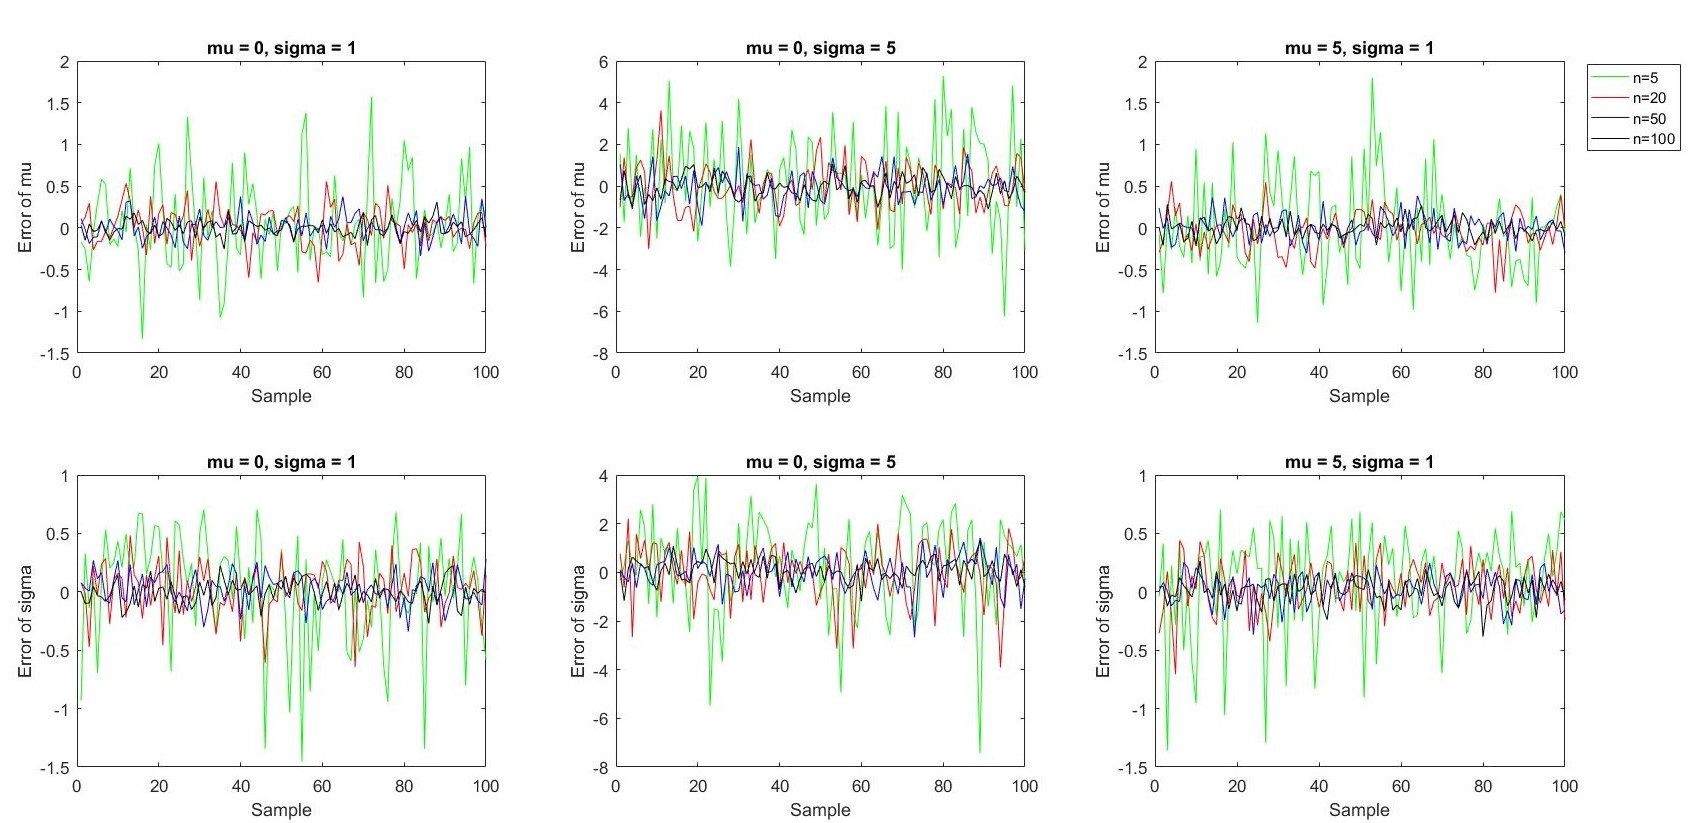
\includegraphics[width = 14.5cm, height = 8cm]{Gumbel.jpg} 
\caption{Plot of Errors of Location and Scale Parameters, MoM}
\label{fig:errorsMoM1}
\end{center}
\end{figure}

\begin{figure}
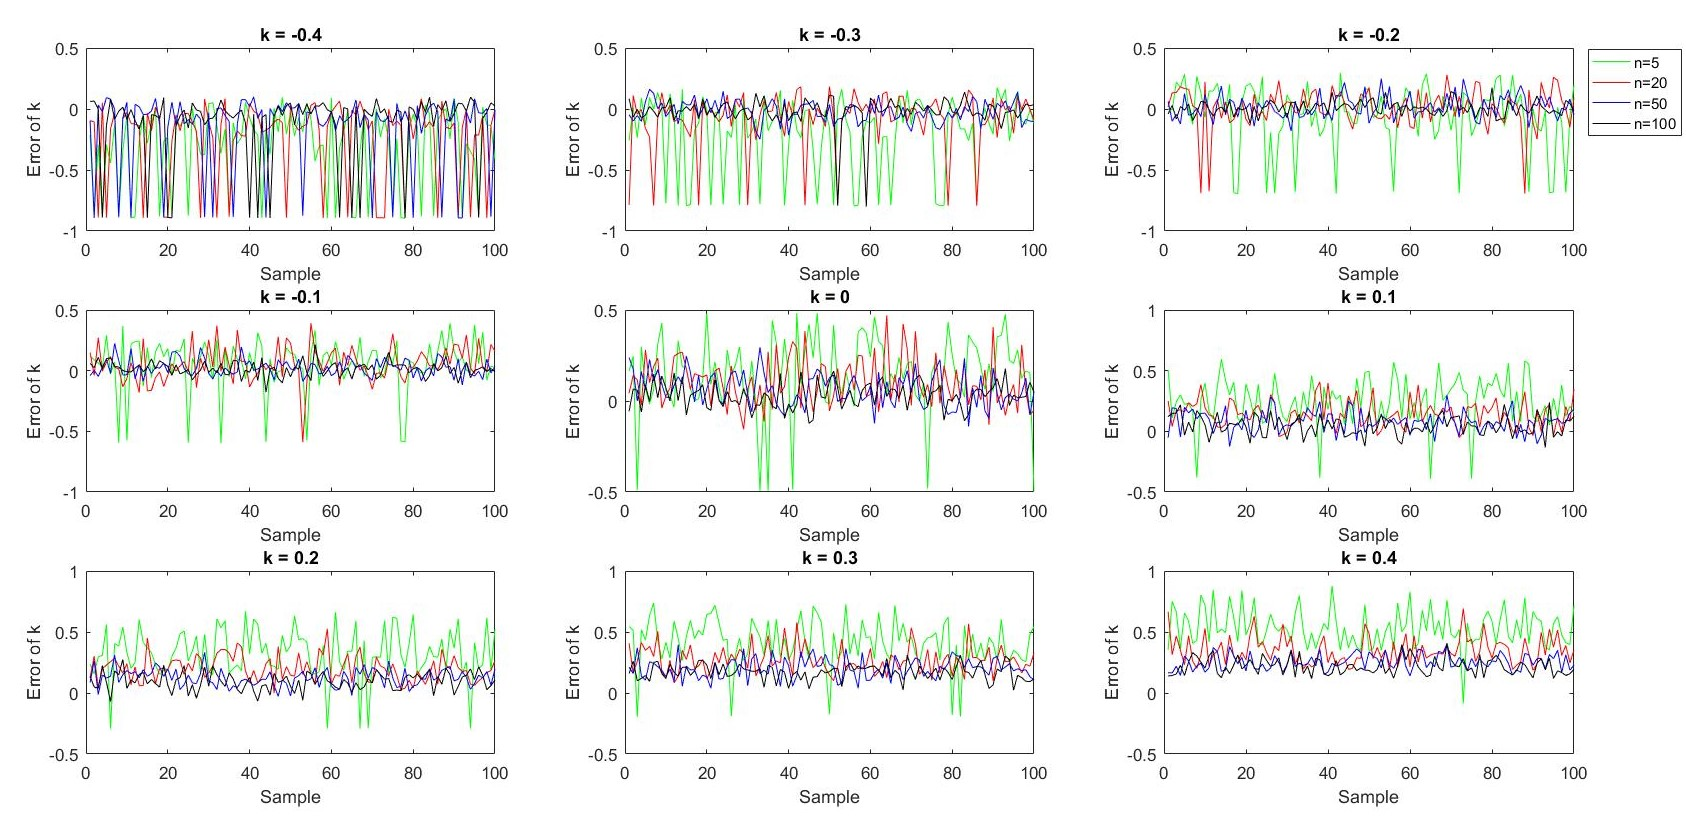
\includegraphics[width = 14.5cm, height = 8cm]{GEV.jpg}
\caption{Plot of Errors of Shape Parameter, MoM}
\label{fig:errorsMoM2}
\end{figure}
% The equations above contain multiple Gamma functions of $\hat{k}$, whose sign is not known. Therefore, to evaluate $\hat{k}$, we require an iterative solution with an initial guess of $\hat{\gamma}$. To avoid this, a simple expression is derived using the following procedure: 
% \begin{enumerate}
% \item For random $k$ values (in a practical range), corresponding values of $\gamma$ are computed from (3). 
% \item The generated sets $(k,\gamma)$ are fitted into a simple function $k=\phi(\gamma,a_{i})$, where $\phi$ is an arbitrary function and $a_{i}$ are some parameters.
% \item The parameters of $\phi$ are determined using the Marquardt (1963) algorithm to give a simple relationship between $k$ and $\gamma$.
% \end{enumerate}

% So, for a known skewness of the sample data, the shape parameter $\hat{k}$ can be computed. The previous procedure is used to yield simple relationships for $\mu$ and $\sigma$, and are given as:
% \paragraph{Relationship between $\hat{\gamma}$ and $\hat{k}$}
% \[ \hat{k} = \begin{cases}
% 0.0087\hat{\gamma}^{3} + 0.0582\hat{\gamma}^{2} - 0.32\hat{\gamma} + 0.2778 & \textrm{for} -0.7 \leq \hat{\gamma} \leq 1.15 \\
% -0.31158\{1-\textrm{exp}[-0.4556(\hat{\gamma}-0.97134)]\} + 1.13828 & \textrm{for} \hspace{3pt} \hat{\gamma} \geq 1.15
% \end{cases} \]
% \paragraph{Relationship between $\hat{\sigma}$ and $\hat{k}$}
% \begin{align*}
% \frac{\hat{\sigma}}{S} = -0.1429\hat{k}^{3} - 0.7631\hat{k}^{2} + 1.0145\hat{k} + 0.779 \hspace{60pt} \textrm{for} -0.5 \leq \hat{k} \leq 0.5
% \end{align*}
%\paragraph{Relationship between $\hat{\mu}$ and $\hat{k}$}
%\[ \frac{\hat{\mu}-\Bar{X}}{S} = \begin{cases}
%0.514075(\hat{k})^{1.33199} - 0.44901 & \textrm{for} \hspace{3pt} 0.01 \leq \hat{k} \leq %0.5 \\
%19.357\hat{k}^{4} + 13.749\hat{k}^{3} + 4.484\hat{k}^{2} + 0.5212\hat{k} - 0.4427 & %\textrm{for} -0.5 \leq \hat{k} \leq 0.01
%\end{cases} \]

%Below is My (Tudor) Work

\newpage
\newpage

\subsection{Maximum Likelihood Estimators (MLEs)}

%References (Castillo, 1988) (Cenac, Mahdi, 2014), (Martins, Stedinger, 2000)

\subsubsection{MLE Estimation for the Gumbel Distribution}

The CDF of the Gumbel distribution is given by $F(X)=\exp(\exp(-(X-\mu)/\sigma)))$, where $\mu$ and $\sigma$ are the location and scale parameters respectively, as usual. Differentiating we can obtain the probability density function:
$$f(X) = \frac{1}{\sigma}\exp\left(-\frac{X-\mu}{\sigma}-\exp\left(-\frac{X-\mu}{\sigma}\right)\right).$$

For a random sample $X_1,\ldots,X_n$ from the previous PDF, the likelihood function is given by
\begin{align*}
    L(\mu,\sigma) &= \prod_{i=1}^{n}f(x),\\
                  &= \sigma^{-n}\exp\left[-\sum_{i=1}^{n}\frac{x_i - \mu}{\sigma}-\sum_{i=1}^{n}\exp\left(-\frac{x_i - \mu}{\sigma}\right)\right].
\end{align*}

Setting $\partial(\log L)/\partial\mu = 0 \text{ and } \partial (\log L)/\partial\sigma = 0 \text{ at } \mu = \hat{\mu} \text{ and } \sigma = \hat{\sigma},$ we obtain after some algebra the equations for the MLEs (Castillo, 1988):
\begin{align}
\hat{\sigma} + \ddfrac{\sum_{i=1}^{n}x_{i}\exp\left(-x_{i}/\hat{\sigma}\right)}{\sum_{i=1}^{n}\exp\left(-x_{i}/\hat{\sigma}\right)} = \bar{x},\label{MLEgumbel1}\\
\hat{\mu} = \hat{\sigma}\log\left[\frac{1}{n}\sum_{i=1}^{n}\exp\left(-\frac{x_{i}}{\hat{\sigma}}\right)\right].\label{MLEgumbel2}
\end{align}

The MLEs $\hat\sigma$ and $\hat\mu$ can be obtained numerically (Mahdi \& Cenac, 2004).

\begin{remark}
$\bar{x} = \frac{1}{n}\sum_{i=1}^{n}x_{i}.$
\end{remark}

\subsubsection{MLE Estimation for the GEV Distribution}

The CDF of the General Extreme Value distribution is given by $F(x)=\exp(-(1-k(x-\mu)/\sigma)^{(1/k)})$ if $k\neq 0$ and $F(x)=\exp(-\exp(-(x-\mu)/\sigma))$ if $k=0.$

If the set $\{X_i\}$ are i.i.d from a GEV distribution, then the log-likelihood function for a sample of n observations $\{x_i\}$ is
\begin{align*}
l(\theta |x)&= \log[L(\theta |x)],\\
			&= -n\log(\sigma) + \sum_{i=1}^{n}\left[\left(\frac{1}{k}-1\right)\log(y_i) -(y_i)^{1/k}\right],
\end{align*}
where $\theta = (\mu,\sigma,k)$ and $y_i= 1-k(x-\mu)/\sigma.$

The MLE of $\mu,\sigma, k$ is obtained by solving the system of equations arising from the equations:
$$\frac{\partial l}{\partial\mu}=0, \quad \frac{\partial l}{\partial\sigma} = 0, \quad \frac{\partial l}{\partial k}=0.$$

Solving gives the following equations: (Stedinger \& Martins, 2000)

\begin{equation}
\frac{1}{\sigma}\sum_{i=1}^{S}\left[\frac{1-k-(y_i)^{1/k}}{y_i}\right]=0,\label{MLEGEV1}\\
\end{equation}
\begin{equation}
-\frac{S}{\sigma} +\frac{1}{\sigma}\sum_{i=1}^{S}\left[\frac{1-k-(y_i)^{1/k}}{y_i}\left(\frac{x_i -\mu}{\sigma}\right)\right] = 0,\label{MLEGEV2}\\
\end{equation}
\begin{equation}
-\frac{1}{k^2}\sum_{i=1}^S\left[\log(y_i)\left(1-k-(y_i)^{1/k}\right) + \frac{1-k-(y_i)^{1/k}}{y_i}k\left(\frac{x_i-\mu}{\sigma}\right)\right]=0.\label{MLEGEV3}
\end{equation}

The equations above can be solved numerically and by an iterative method (Newton-Raphson method). It can be noted that the MLE equations for the GEV are significantly more complex than the MLE equations for the Gumbel.

%\newpage

\subsubsection{Working with MLEs}

In practice, when evaluating MLEs of Gumbel and GEV distributions, we use the \textit{evfit(X)} and \textit{gevfit(X)} functions in MATLAB, where X is the data.

As seen in the MATLAB documentation: `parmhat = evfit(data) returns maximum likelihood estimates of the parameters of the type 1 extreme value distribution given the data in the vector data. parmhat(1) is the location parameter, mu, and parmhat(2) is the scale parameter, sigma.' and `parmhat = gevfit(X) returns maximum likelihood estimates of the parameters for the generalized extreme value (GEV) distribution given the data in X. parmhat(1) is the shape parameter, k, parmhat(2) is the scale parameter, sigma, and parmhat(3) is the location parameter, mu.' (MathWorks, 2018a and 2018b)

%%%%%%%%%%%%%%%%%%%%%%%%%%%%%%%%%%  Submitted by Nishant - 12/06/2018 below
\subsection{Probability-Weighted Moments (PWM)}

Probability-weighted moments are a generalised version of standard moments of a probability distribution. According to Hosking et al. (1985), they were introduced by Greenwood et al. (1979). PWM have desirable properties which will be discussed further and they provide convenient parameter estimation for a variety of distributions including the logistic, Weibull and Gumbel - and are especially useful for estimation with a small sample.

\subsubsection{Introduction to PWM}
Suppose we have a random variable $X$ with distribution function $F$. Probability-weighted moments are given by:

\begin{align}
M_{p,r,s} = E[X^p\{F(X)\}^r\{1 - F(X)\}^s].
\end{align}
Here we have $p, r, s \in \mathbb{R} $. 

If the inverse distribution function $x(F)$ can be written in closed form it may be more convenient to evaluate these moments using the following:

\begin{align}
M_{p,r,s} = \int_{0}^{1} \{x(F)\}^p F^r (1-F)^s dF.
\end{align}

Notice that $M_{p,0,0}$ are the standard moments of X.

Often it is useful to set $p=1$ as this allows for a simpler calculation and when $r,s$ are integers it is useful to either consider $M_{1,r,0}$ or $M_{1,0,s}$. For the Generalised Extreme-Value and Gumbel distributions with a sample of size n, it is only necessary to consider the following:
\begin{align*}
\beta_r = M_{1,r,0}  = E[X\{F(X)\}^r], \qquad r \in \{0, 1, 2, \ldots n\},
\end{align*}
as suggested by Hosking et al. (1985). Note here that although we can have $p, r, s \in \mathbb{R} $, it is difficult to find estimators for $M_{p,r,s}$ - using $\beta_r$ is preferable since it has simpler estimators. 

Suppose we have a random sample of size n from $F$, we may choose to use an ordered sample $X_{(1)} \leq X_{(2)} \leq X_{(3)} \leq \ldots \leq X_{(n)}$ for estimation of $\beta_r$. The statistic:

\begin{align*}
b_r = \frac{1}{n} \sum_{i = 1}^n \frac{(i-1)(i-2) \ldots (i-r)}{(n-1)(n-2) \ldots (n-r)} x_{(i)},
\end{align*}
is unbiased for $\beta_r$ (Greenwood et al. 1979). Alternatively one can estimate using the following:
\begin{align*}
\hat{\beta}_r = \frac{1}{n} \sum_{i=1}^n p_{i,n}^r\ x_{(i)},
\end{align*}
where $p_{i,n}$ has to be reasonably chosen. Taking $p_{i,n} = (i-a)/n,\ 0<a<1$ gives a consistent estimator $\hat{\beta}_r$ of $\beta_r$. (Hosking et al. 1985)

\subsubsection{PWM Estimation for the Gumbel Distribution}

We have already seen the Gumbel distribution, which is given by equation (1). The Gumbel has a closed form inverse distribution function. This allows for an easier calculation of $\beta_r$. The inverse distribution function $x(F)$ is given by
\begin{align}
x(F) &= \mu - \sigma  \left [\log (-\log F)\right].
\end{align}

This is used for the the computation of the rth order PWM $\beta_r$
\begin{align}
\beta_r = \int_0^1 x(F) F^r dF = \frac{1}{r+1} [\mu + \sigma\{\gamma + \log(r+1)\}]. \label{betargumbel}
\end{align}

Here $\gamma$ is the Euler-Mascheroni constant. It is defined by:
$$\gamma = \lim_{n\to\infty} \left ( \sum_{k=1}^n \frac{1}{k} - \log n \right ) = 0.5772\ldots \ . $$
The result \eqref{betargumbel} arises from substitutions $u = -\log f$ and $m = (r+1)u$.

To determine $\mu, \sigma$ another equation is required. This can be done simply by defining $\beta_q, \quad q\neq r$ in the same way. The result is two relatively straightforward equations which can be manipulated to give:
\begin{align}
\sigma &= \frac{(r+1)\beta_r - (q+1)\beta_q}{\log(r+1) - \log(q+1)}, \\
\nonumber \\
\mu &= (r+1)\beta_r - \sigma[\log(r+1) + \gamma].
\end{align}

For simplicity, let $(r,q) = (0,1)$ and replace $\beta_r$ with an estimator. Here we replace with the consistent estimator $\hat{\beta}_r$ where $p_{i,n} = (i-0.35)/n$ as suggested by Hosking et al. (1985) for estimation of the Generalised-Extreme Value distribution. In their paper for parameter estimation of the Gumbel distribution - (Mahdi \& Cenac, 2003) suggest using the unbiased estimator $b_r$. Nonetheless we follow the suggestion by Hosking since later we use the consistent estimator for parameter estimation of the GEV. 

Thus the following estimators are obtained:
\begin{align}
\hat{\sigma} &= \frac{2\hat{\beta}_1 - \hat{\beta}_0}{\log 2} \label{sigmagumbel},\\
\nonumber \\
\hat{\mu} &= \hat{\beta}_0 - \hat{\sigma}\gamma \label{mugumbel}.
\end{align}

Here \eqref{sigmagumbel} and \eqref{mugumbel} define the classical PWM estimators for the Gumbel distribution (Rasmussen \& Gautam, 2003).

\begin{remark}
When implementing equation \eqref{mugumbel} it was necessary to change the equation for the estimator to work. The equation used was $\hat{\mu} = \hat{\beta}_0 + \hat{\sigma}\gamma$. 
\end{remark}

\subsubsection{PWM Estimation for the GEV Distribution}

The CDF of a GEV distribution is given by equation (4). Importantly, for the calculations, the GEV distribution has a closed form inverse distribution function:

\begin{align}
x(F) &= \mu + \sigma  \left [\frac{1 - (-\log F)^k}{k} \right ] , &k &\neq 0 \\
&= \mu - \sigma  \left [\log (-\log F)\right], &k&=0 \nonumber
\end{align}

Now the calculation of $\beta_r$:
\begingroup
\allowdisplaybreaks
\begin{align}
\beta_r &= M_{1,r,0}, \nonumber \\
&= \bigintssss_0^1 \left[ \mu + \sigma  \left \{\frac{1 - (-\log F)^k}{k} \right \} \right] F^r \ dF, \nonumber \\
\text{Let $u = -\log F$}, \nonumber \\
&= \bigintssss_0^{\infty} \left[ \mu + \sigma \left\{\frac{1-u^k}{k}\right \} \right] \textit{e}^{-(r+1)u} \ du, \nonumber \\
\nonumber \\
&= \left(\mu + \frac{\sigma}{k} \right) \bigintssss_0^{\infty} \textit{e}^{-(r+1)u} \ du - \frac{\sigma}{k} \bigintssss_0^{\infty} u^k \textit{e}^{-(r+1)u} \ du, \nonumber \\
\nonumber \\
&= \left(\mu + \frac{\sigma}{k} \right)(r+1)^{-1} - \frac{\sigma}{k} \left( r+1 \right)^{-1-k} \ \Gamma (1+k), \nonumber \\
\nonumber \\
\Rightarrow \beta_r &= (r+1)^{-1} \left [\mu + \frac{\sigma \{ 1 - (r+1)^{-k} \ \Gamma(1+k)\}}{k} \right], \quad \text{if }k > -1.\label{beta}
\end{align}
\endgroup
If $k \leq -1$, $\beta_r$ does not exist. 

Now that \eqref{beta} gives us the equation of $\beta_r$, it is necessary to manipulate this into yielding values for $\mu, \sigma, k$. Using \eqref{beta} the following equations hold:

\begin{align}
\beta_0 &= \mu + \frac{\sigma \{ 1 - \Gamma(1+k)\}}{k}, \\
\nonumber \\
2\beta_1 - \beta_0 &= \frac{\sigma \Gamma(1+k)(1-2^{-k})}{k}, \\
\nonumber \\
\frac{3\beta_2 - \beta_0}{2\beta_1 - \beta_0} &= \frac{1 - 3^{-k}}{1 - 2^{-k}}. \label{keqn}
\end{align}

Note here that the probability-weighted moments used are $r = 0, 1, 2$. We do not want the higher deviation from using bigger r values. Also using the lowest values to get three equations for three unknowns allows for a simpler solution.

To yield the estimators $\hat{\mu}, \hat{\sigma}, \hat{k}$, the quantity $\beta_r$ must be replaced by an estimator, either $\hat{\beta}_r$ or $b_r$. Hosking et al. (1985) suggests using the consistent estimator $\hat{\beta}_r$ where $p_i,n = (i-0.35)/n$ for the best performance. Using the unbiased estimator $b_r$ is not always ideal since it has a higher variance.
\begin{align}
\frac{3\hat{\beta}_2 - \hat{\beta}_0 }{2\hat{\beta}_1 - \hat{\beta}_0 } = \frac{1 - 3^{-\hat{k}}}{1 - 2^{-\hat{k}}} \label{khateqnunsol}
\end{align}

To solve \eqref{khateqnunsol} for $\hat{k}$ we require iterative methods. Since $(1 - 3^{-\hat{k}})/(1 - 2^{-\hat{k}})$ is almost linear over the range $   -1/2< \hat{k} < 1/2 $, which are the values most commonly seen in practice; Hosking et al. (1985) suggest that low-order polynomial approximations are accurate enough. They propose the following estimator:
\begin{align}
\hat{k} = 7.859c + 2.9554c^2, \qquad c = \frac{2\hat{\beta}_1 - \hat{\beta}_0}{3\hat{\beta}_2 - \hat{\beta}_0} -\frac{\log 2}{\log 3}. \label{khateqn}
\end{align}

Then using $\hat{k}$, estimators for $\sigma$ and $\mu$ can be found:
\begin{align}
\hat{\sigma} &= \frac{(2\hat{\beta}_1 - \hat{\beta}_0)\hat{k}}{\Gamma(1+\hat{k})(1 - 2^{-\hat{k}} )}, \label{sigmahateqn} \\
\nonumber \\
\hat{\mu} &= \hat{\beta}_0 + \frac{\hat{\sigma} \{\Gamma(1+\hat{k}) - 1 \} }{\hat{k}}. \label{muhateqn}
\end{align}

Here the equations \eqref{khateqn}, \eqref{sigmahateqn} and \eqref{muhateqn} define PWM estimators of the GEV distribution.

\begin{remark}
When implementing equation \eqref{muhateqn} it was necessary to change the equation for the estimator to work. Instead $-\hat{k}$ was used in the code.   
\end{remark}

\subsubsection{Properties and Performance of the PWM Estimator}
\
%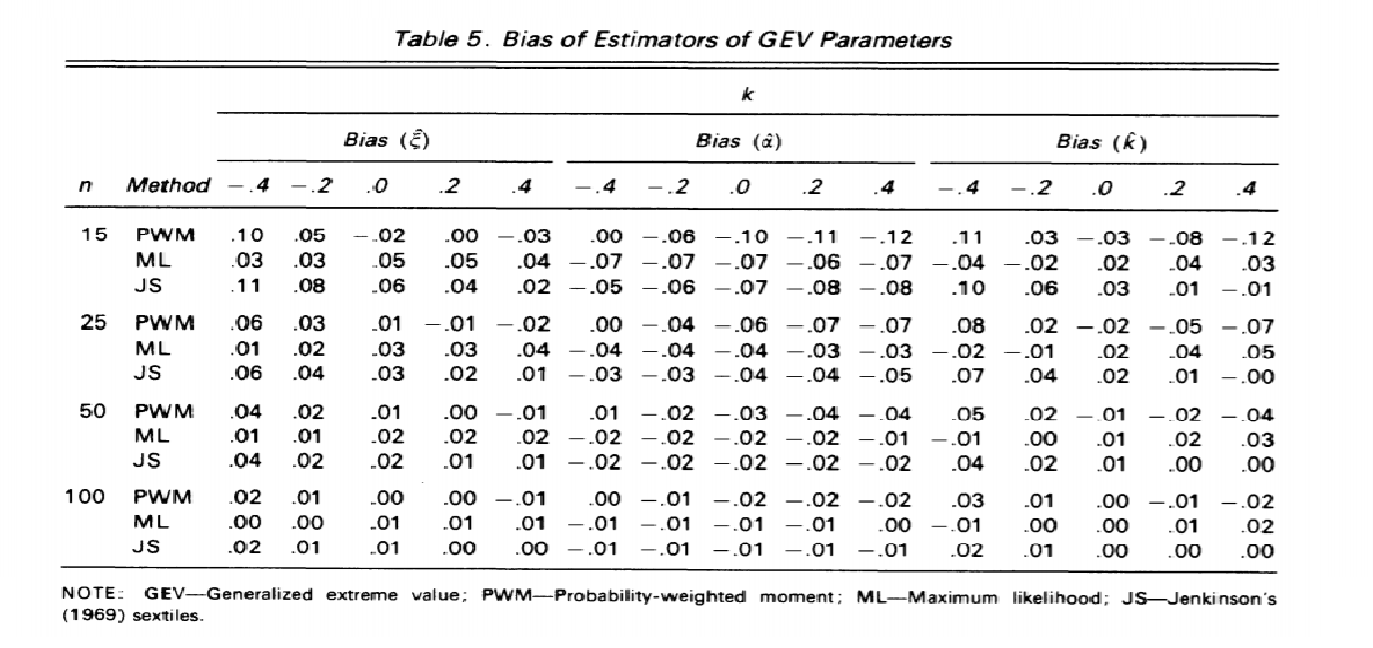
\includegraphics{HoskingBias.png}
%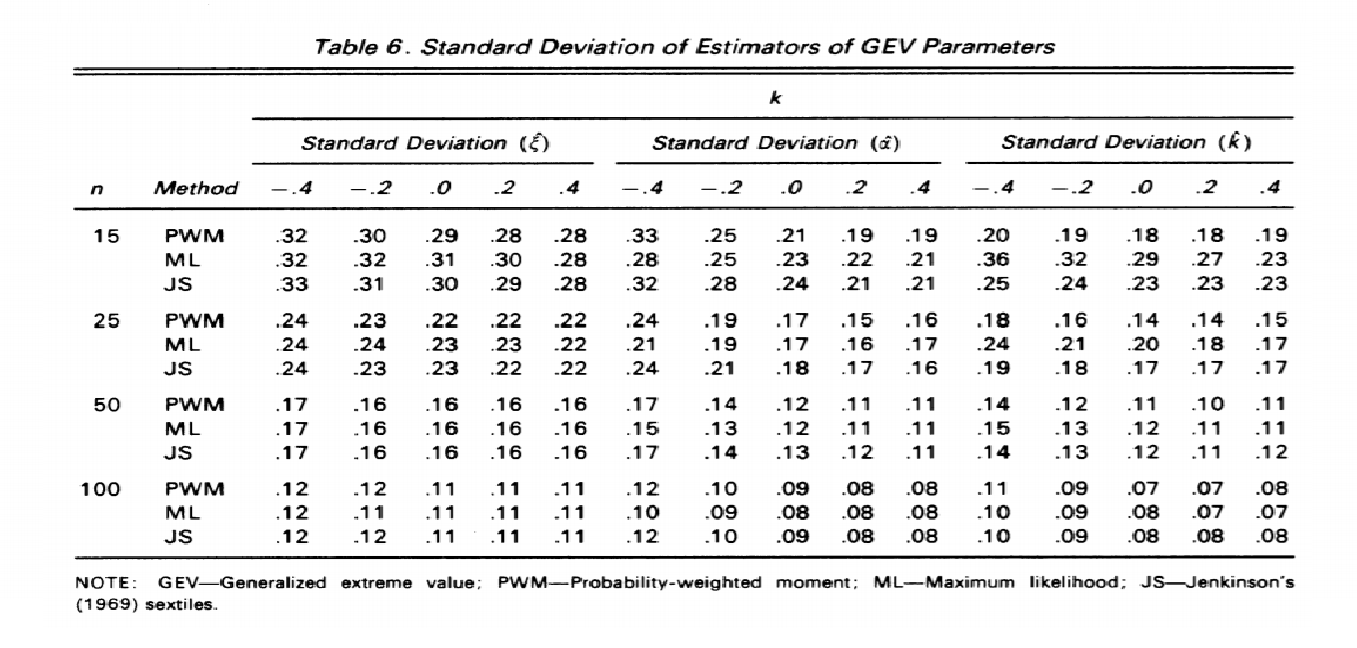
\includegraphics{HoskingSD.png}
%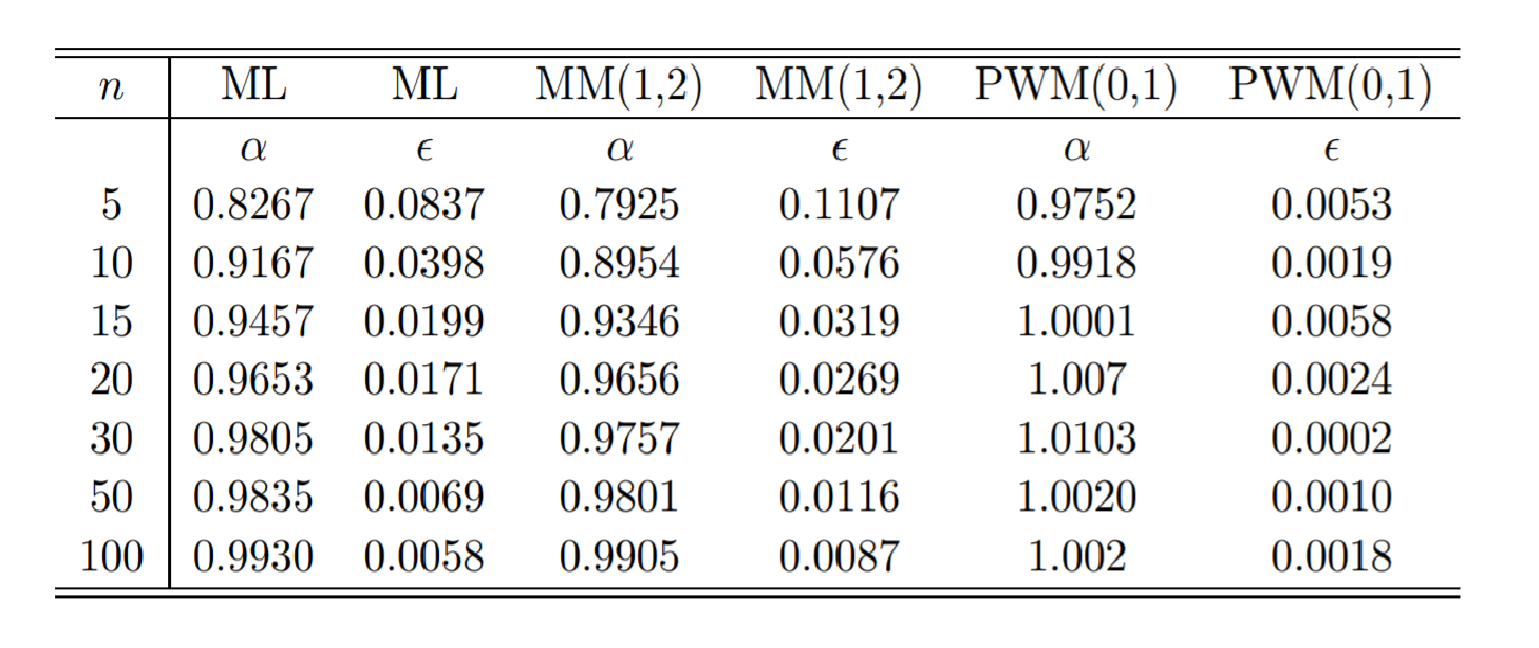
\includegraphics{MahdiEstimates.png}

PWM estimates of the GEV distribution satisfy criteria, that $\hat{k} > 1$ and that $\hat{\sigma} > 0$. These are desirable properties especially since in practice, $-1/2 < k < 1/2$, and it is important to have a positive scale parameter, $\sigma$. For the proof see (Hosking et al. 1985).

The PWM and MLE methods discussed in this report are invariant under linear transformation (Hosking et al. 1985) - thus to assess performance it is conventional and convenient to set $\mu = 0$ and $\sigma = 1$ for the GEV and Gumbel distributions and allow the shape $k$ to vary for the GEV distribution.

The PWM has come under criticism  since the method assumes \textit{a priori} that $k<1$, which can be seen by manipulating \eqref{beta}. Further this implies that the distribution has a finite mean. However the GEV distribution is defined $\forall \ k \in \mathbb{R}$. To broaden the domain of the shape $k$ for PWM, a new class of moments called GPWM (generalised probability-weighted moments) has been introduced. This adds a suitable continuous function $\omega$ to the definition. Although this massively increases complexity it allows for a wider domain of $k$ for which these moments can be computed.\\

\underline{\textbf{Gumbel Estimation:}}

Here we discuss PWM estimator performance for the Gumbel distribution.

To see the performance of PWM estimators and compare them with MoM estimators and MLEs we use data from (Mahdi \& Cenac, 2004). They computed empirical estimates from a random sample of different sizes (which they denote n) of the standard Gumbel distribution with $\mu = 0, \sigma = 1$. They denote the scale by $\alpha$ and the location by $\epsilon$. For PWM they used (r, q) = (0, 1) to use the classical estimators and elected to use the unbiased estimator $b_r$ (Greemwood et al. 1979) for $\beta_r$. For MoM - they elected to use the $1^{\text{st}}$ and $2^{\text{nd}}$ moments.

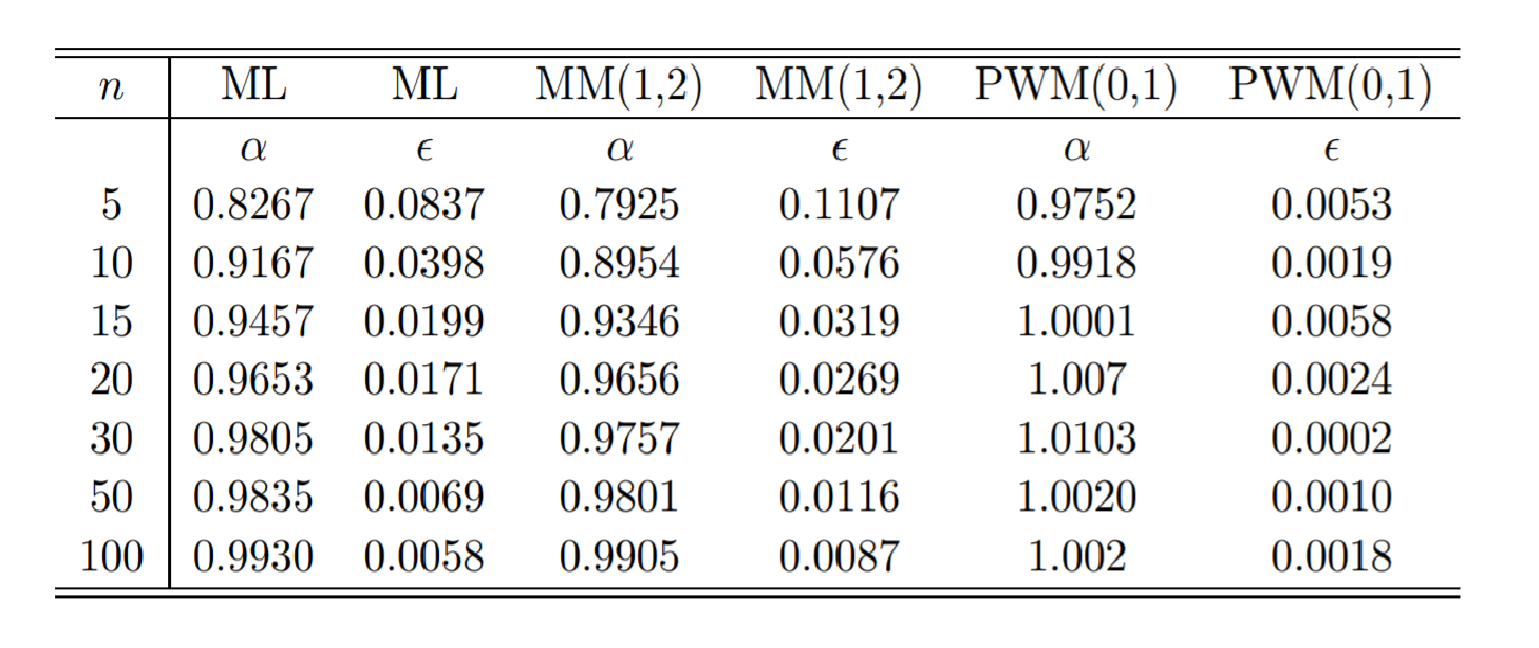
\includegraphics[width = 1 \textwidth, height = 4.4cm]{MahdiEstimates.png}\vspace{-0.5cm}

\small{Table of empirical estimates of scale and location using the MoM, PWM and ML methods for the standard Gumbel distribution. (Mahdi \& Cenac, 2004: p.5)}\vspace{-0.2cm}

\normalsize
As can be seen the PWM estimates are far better than MoM and MLE for small to moderate samples. All three methods perform well for large samples. Although we use this for our example - for the Gumbel distribution - using the classical PWM estimators does not provide the best performance. (Mahdi \& Cenac, 2004) suggest using low values for $(r,q)$ to avoid over-weighting large sample observations. A method suggested by (Rasmussen \& Gautam, 2003) eliminates $q$ by studying the effects of when $q \to r$ using L'H$\hat{\text{o}}$pital's Rule, computing an estimator based solely on $r$ and then using an empirical relationship to best choose $r$. It provides an improvement of approximately 10\%.\vspace{-0.2cm}


%%%% BELOW PLEASE LEAVE AS IT IS AS OTHERWISE LEGEND OF THE TABLE BELOW GOES OVER THE PAGE

\underline{\textbf{GEV Estimation:}}\vspace{-0.2cm}

Here we discuss PWM estimator performance for the Generalised Extreme-Value distribution. To see the performance for the GEV distribution we use data from Hosking et al. (1985). Here the scale and location parameter have been set to 1 and 0 respectively. For comparison they  use different values for shape $k$ for the distribution using $k = -0.4, -0.2, 0, 0.2, 0.4$. The use a variety of sample sizes n and they compare three methods: PWM, MLE and Jenkinson's method of sextiles (JS) - which is not discussed here. For the PWM they elected to use the consistent estimator $\hat{\beta}_r$ where $p_{i,n} = (i-0.35)/n$ which was chosen since it gave the best overall results. In terms of notation scale is denoted $\alpha$ and location is denoted $\xi$. The bias and standard deviation of the estimators for the GEV parameters are shown: 

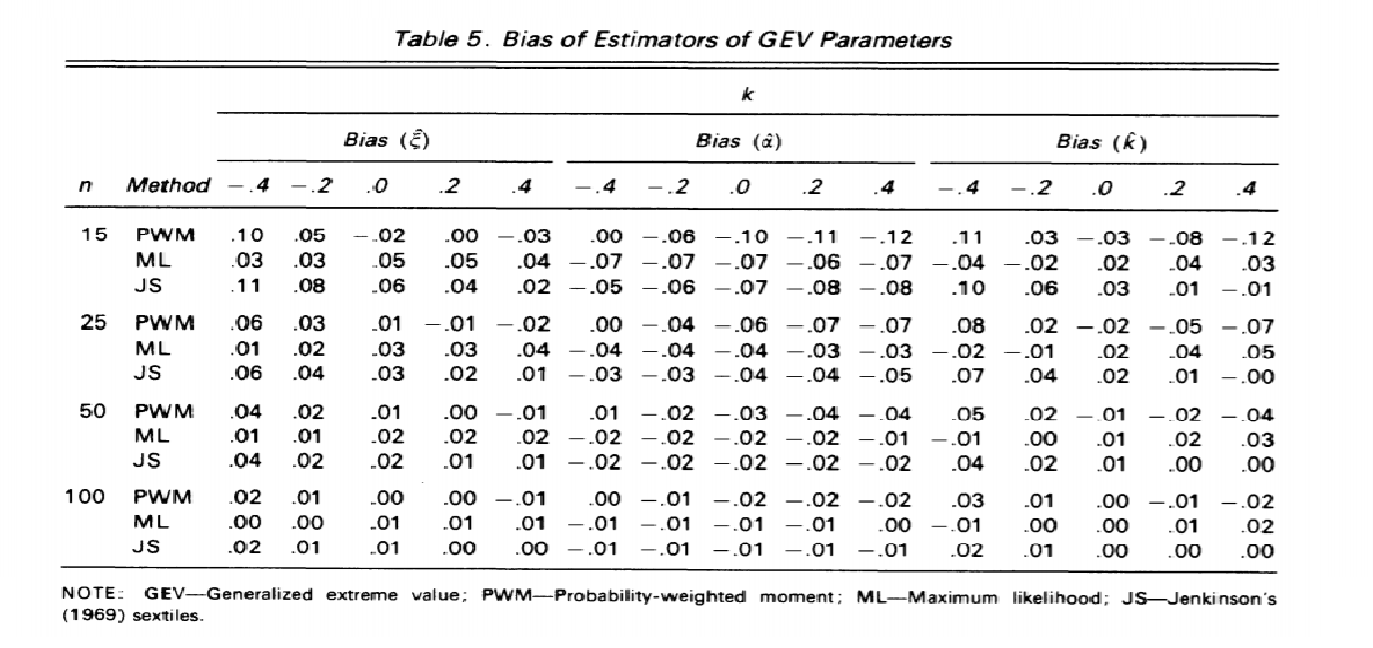
\includegraphics[width = 1 \textwidth]{HoskingBias.png}
\small{Table showing the bias of estimators for the GEV parameters for different values of $k$ from a GEV distribution with $\mu = 0$ and $\sigma = 0$. \ (Hosking et al. 1985: p.8)}\normalsize

\hspace{-0.8cm}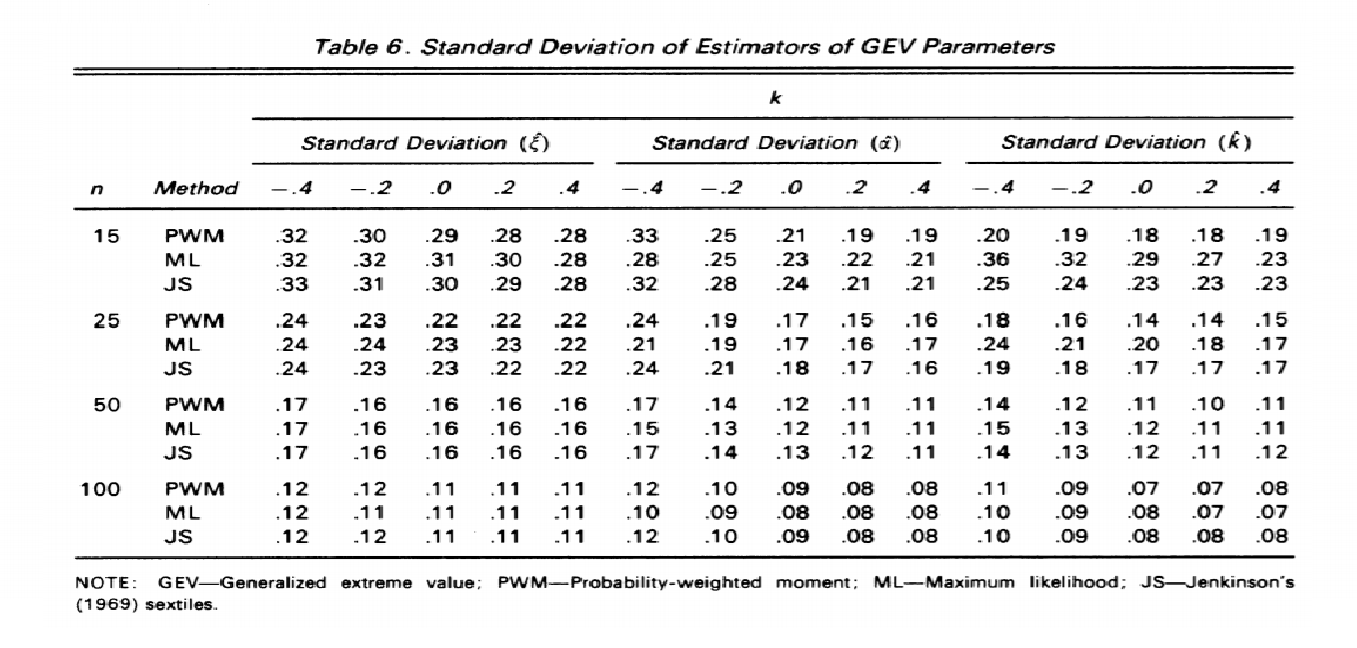
\includegraphics[width = 1.1 \textwidth]{HoskingSD.png}
\small{Table showing the standard deviation of estimators for the GEV parameters for different values of $k$ from a GEV distribution with $\mu = 0$ and $\sigma = 0$. \ (Hosking et al. 1985: p.8)}\normalsize
\vspace{0.5cm}


In general, it can be seen that the PWM estimator for $k$ has a larger bias than the ML estimator, however this is small near the important value when $k=0$. Where the advantage of PWM lies is in the low standard deviation particularly for small samples, $n=15$ and $n=25$. The bias is relatively insignificant compared to the standard deviation when calculating the mean square error of $\hat{k}$.

With regards to estimators for $\mu$ and $\sigma$ similar results can be seen. Generally, PWM estimators have smaller standard deviation especially for small samples and their bias, although larger than ML (which have the lowest bias in this example), is not enough to significantly impact mean square error. (Hosking et al. 1985)

\underline{\textbf{Conclusion:}}

PWM offers  a fast and straightforward way of computing feasible estimated parameters of both the GEV and Gumbel distributions. They perform better than MLEs for small samples and although tend to have a higher bias, these decrease quickly as the sample size increases. (Hosking et al. 1985). The most useful property of PWM estimators is its low standard deviation which is comparable with MLEs for large samples and far smaller for small samples. This allows for a smaller MSE (mean squared error).

%%%%%%%%%%%%%%%%%%%%%%%%%%%%%%%%%%%%%%%%%%%%%%%%%%%%%%%%%%%%%%%%%%%%%%%%%%%%%%%%%%%%%%

\newpage

\section{Goodness of Fit}
\subsection{Quantile-Quantile Plots}
\underline{\textbf{Construction:}}

A Quantile-Quantile plot (QQ plot) is a graphical method to determine whether two data sets are from the same distribution, with an emphasis on fitting the tails. As the goodness of fit is tested for an Extreme Value distribution, order statistics and theoretical quantiles will used as the two data sets. No assumptions are made on the distribution of the sample data. Gumbel and Generalised Extreme Value (GEV) distribution will be compared to the data of the maxima by the following method: (Scott, 2018)

Let $Z_1,\ldots, Z_M$ denote M observations of the maximum value:\vspace{-0.2cm}
\begin{enumerate}
  \item \textbf{Ordered Statistics, $z_{(i)}$:} \\ The random sample, ${z_1, z_2,\ldots, z_M}$, is used to create the order statistics so: 
  \vspace*{-3mm}
  \begin{flushleft}
   $z_{(1)} < z_{(2)} <\ldots< z_{(M-1)} < z_{(M)},$ 
  \end{flushleft}
    \vspace*{-3mm}
   These M ordered values will form the input sample quantiles, $z_{(i)}$ so:
   \vspace*{-3mm}
   \begin{center}
   $F(z_{(i)}) \approx i/M, \text{ where}$
   \end{center}
   \vspace*{-3mm}
  $z_{(i)}$ - order statistic, 
  $i/M$ - probability associated with each $z_{(i)}$,
  $F$ - empirical distribution.

  \item \textbf{Theoretical Quantiles, $y_i$:} \\ The distribution curve, either Gumbel or GEV distribution, will be divided M times into M+1 quantiles, each with equal probability.
  \vspace*{-3mm}
  \begin{center}
  $\hat{F}$$(y_i) = p_i$ 
  \end{center} 
  \vspace*{-3mm}
  $y_i$ - theoretical quantiles, 
  $p_i$ - probability associated with each $y_i$, \\
  $\hat{F}$ - Gumbel or GEV distribution with estimated parameters. \\
 \\ $p_i$ is set as $(i-1/2)/M$ to avoid discrepancies: suppose if $p_i = i/M$ and $i = M$, then $\hat{F}$$(y_M) = 1$.
  
   \begin{figure}[h]
    \centering
    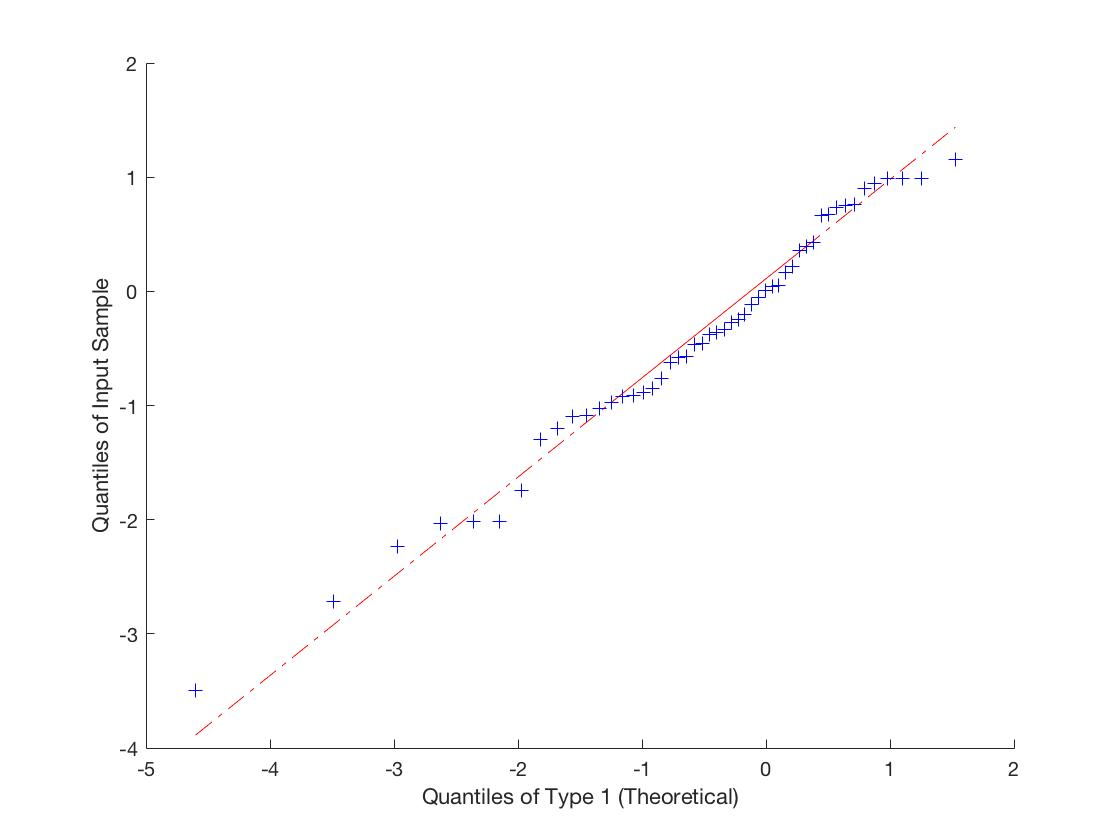
\includegraphics[width=9cm]{qqgeneral.png}
  \vspace*{-5mm} 
  \caption{Example of a QQ Plot: Random Sample of 50 from Gumbel distribution}
  \label{qqplotexample}
  \end{figure}
\end{enumerate}  

\underline{\textbf{Interpretation of QQ Plots:}}

A QQ plot has a reference line plotted; the data points needs to be approximately on this line, so that the data sets come from the same distribution. If $y_i$ and $z_{(i)}$ are identically distributed, the QQ plot will be a 45$^{\circ}$ straight line, with gradient 1, passing through the origin.

This straight line may vary in gradient and y-axis intercept for various data sets, given $y_i$ is a linear function of $z_{(i)}$. This occurs when the data is not standardised, so an alternative straight line is plotted, $z_{(i)} = (y_i - \mu)/\sigma$, where $\mu$ is the estimated location parameter and $\sigma$ is the estimated scale parameter. (Wilk \&  Gnanadesikan, 1968)

QQ plots may indicate departure from the theoretical distribution. This occurs if the data is skewed or has large kurtosis. (Scott, 2018)
 \vspace*{-2mm} 
\begin{figure}[h]
 \centering
    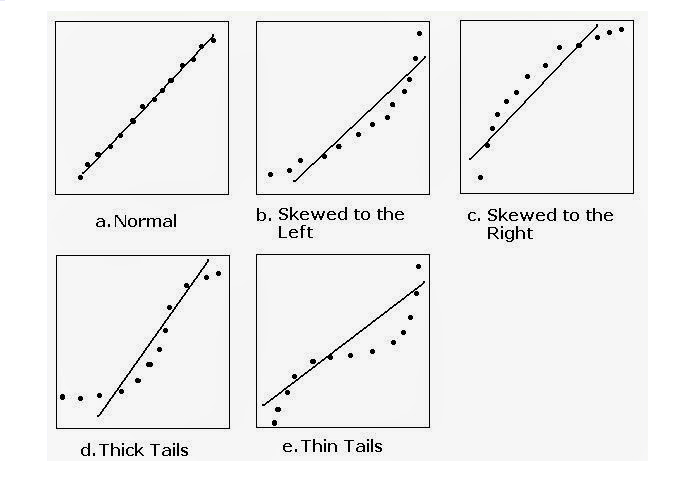
\includegraphics[width=8cm]{skewtails.png}
  \vspace*{-5mm} 
  \caption{Departures in QQ Plots (Jost, 2018)}
  \label{departuresinqqplots}
  \end{figure}

\underline{\textbf{Simulating Samples from Gumbel and Generalised Extreme Value Distribution:}} 
 
The sample quantiles are a random sample from the Extreme Value distribution (Gumbel or GEV). The theoretical quantiles are formed from the same distribution. The deviation of the generated QQ plots will be observed, thereby determining the usefulness of this test. 
 
\begin{figure}
\centering
\begin{subfigure}
  \centering
  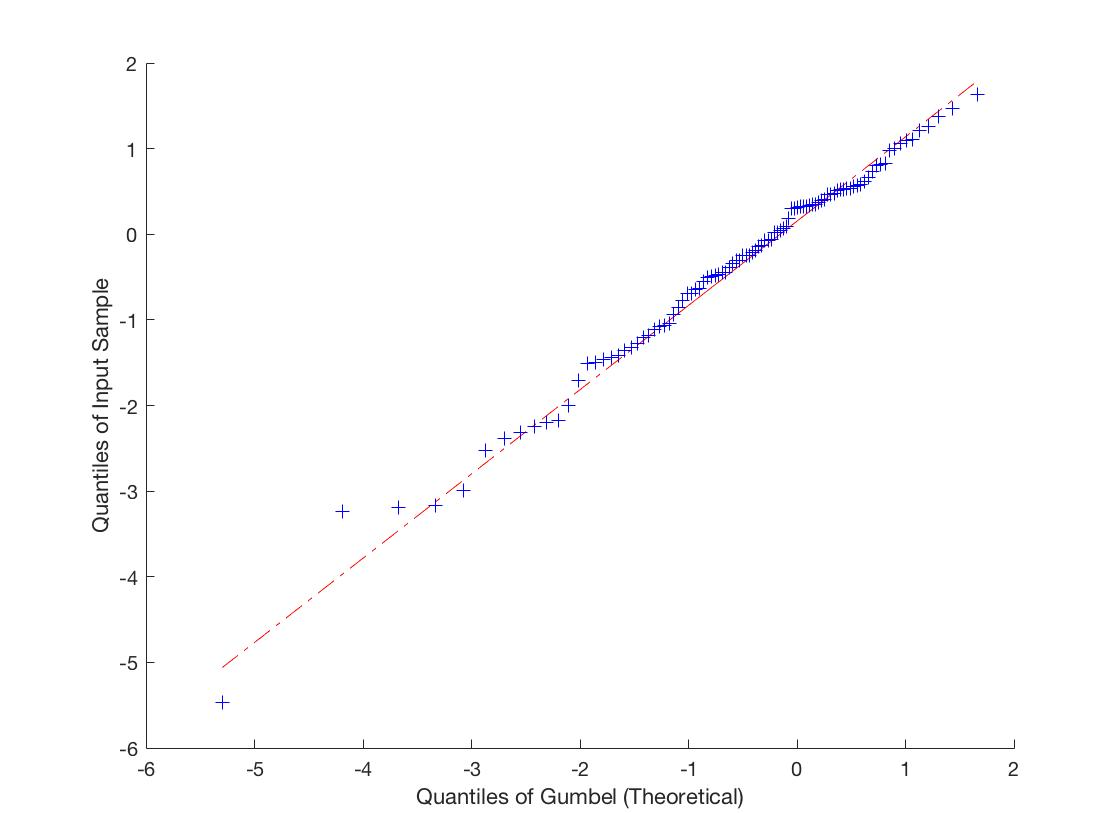
\includegraphics[width=6.5cm]{EVQQ1.png}
\end{subfigure}
\begin{subfigure}
  \centering
  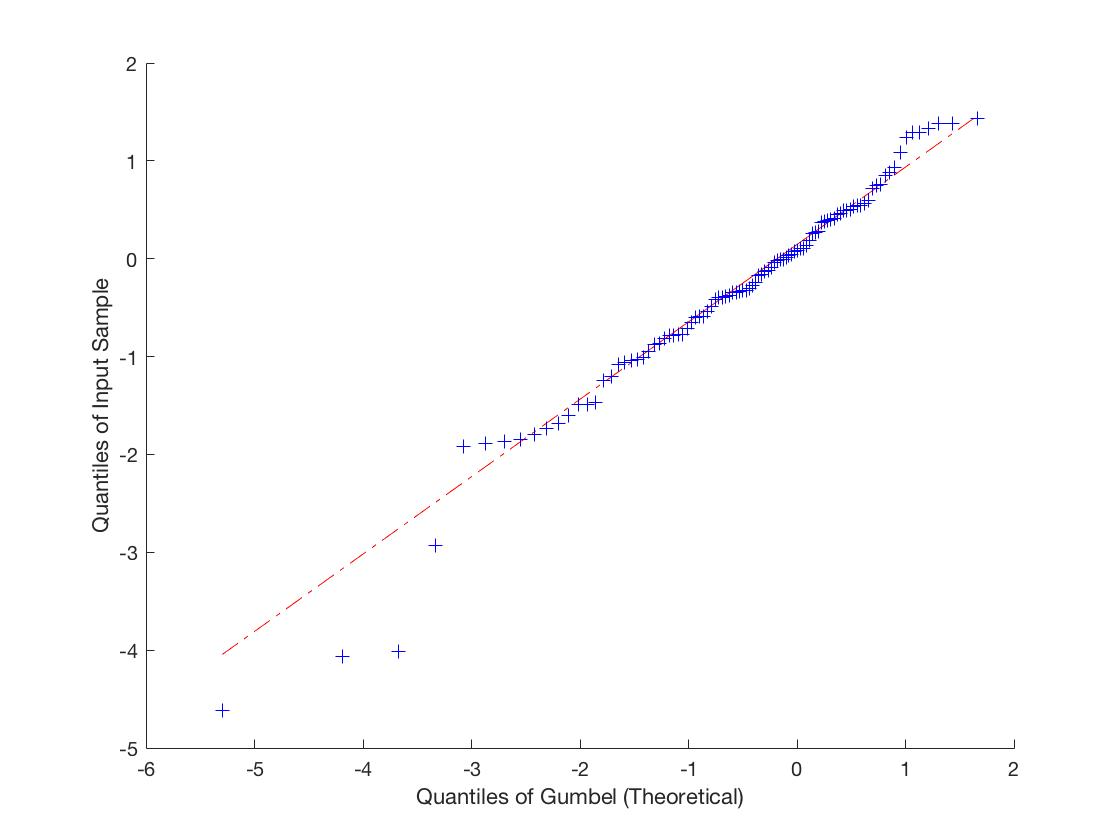
\includegraphics[width=6.5cm]{EVQQ2.png}
\end{subfigure}
  \vspace*{-5mm} 
\caption{Gumbel QQ Plots}
\label{gumbelqqplots}
\end{figure}
\begin{figure}
\centering
\begin{subfigure}
  \centering
  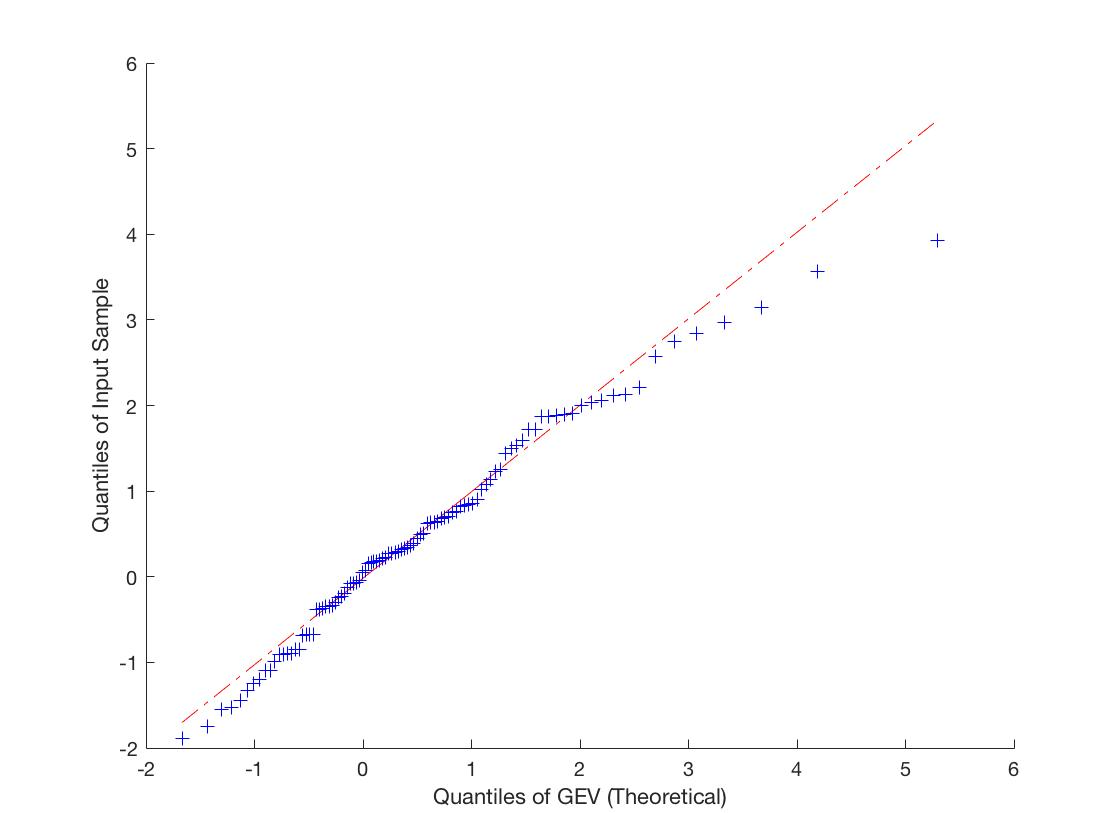
\includegraphics[width=6.5cm]{GEVQQ1.png}
\end{subfigure}
\begin{subfigure}
  \centering
  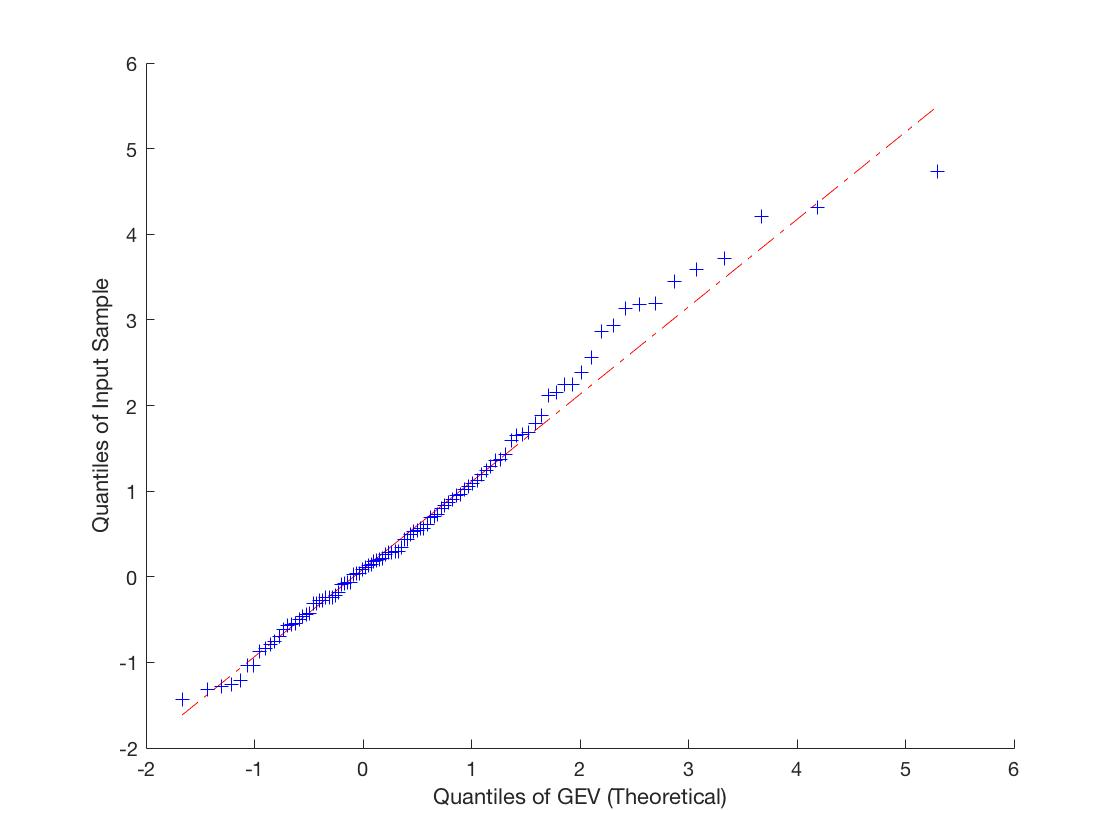
\includegraphics[width=6.5cm]{GEVQQ2.png}
\end{subfigure}
  \vspace*{-5mm} 
\caption{GEV QQ Plots}
\label{gevqqplots}
\end{figure}

QQ plots vary from sample to sample - the plots below are of size 100, which is similar to the sample size used in the worked example later.

Gumbel and GEV are sampled using $gevrnd$ and $evrnd$ respectively on MATLAB, with parameters: $\sigma = 1$, $\mu = 0$ and $k = 0$ (for $gevrnd$ only). The points will approximately lie on a $45^{\circ}$ straight line if the input sample matches the distribution. In order to not reject a distribution, the points need to be randomly scattered, not having kurtosis or a skew. Outliers are easy to spot in QQ plots.

In both the plots of Figure \ref{gumbelqqplots}, the majority of the data points fit $y = x$, but the first 3 sample quantiles appear to not fit the Gumbel distribution. These can be taken as outliers as there appears to have no skew or large kurtosis, hence the input sample follows the Gumbel distribution.

The first plot of Figure \ref{gevqqplots} is skewed slightly to the right, thereby suggesting the sample size of 100 does not fit the GEV distribution. However, the data points aside from the last 4 sample quantiles (outliers) lie closely to the $y = x$ reference line. The other QQ plots approximately lie on $y=x$, so follow the given distribution.

The variations observed in the QQ plots are not significant enough to rule out the distribution that the input sample is compared to. Therefore, a QQ plot is effective in determining whether the input sample follows a certain distribution. 

\subsection{Parametric Bootstrap} 

Parametric bootstrap is another goodness of fit test for distributions with estimated parameters, which relies on sample with replacement. In a general sense, it finds properties of an estimator.

Define: (Babu, 2011)

$\{F(\ \cdot \ ; \theta): \theta \in \Theta\}$ - a family of continuous distributions,

$\Theta$ - parameter space, an open region in \textit{p}-dimensional space,

$F^{*}$ - empirical distribution,

$x_1,\ldots,x_n$ - sample data of size n,  

$x^{*}_1,\ldots, x^{*}_n$ - resample of size n,

$u$ - statistic computed from the sample,

$u^{*}$ - statistic computed from the resample.

The Bootstrap principle says (Orloff \& Bloom, 2014):
\begin{itemize}
  \item $F^{*} \approx F$.
  \item The variation of $u$ can be predicted by variation of $u^{*}$.
\end{itemize}

\underline{\textbf{Construction:}}

Parametric bootstrap involves generating a bootstrap sample to estimate a confidence interval for an unknown parameter, $\theta$ through the bootstrap difference.

The method is as follows: (Orloff \& Bloom, 2014)
\begin{enumerate}
  \item $x_1,\ldots,x_n$ is a data sample for $F(\theta)$.
  \item Statistic, $\hat{\theta}$, is used to estimate $\theta$ through parameter estimation methods, which was covered in Section 4.
  \item $x^{*}_1,\ldots,x^{*}_n$ is a resample of the data with replacement from the empirical distribution, $F^{*}$. The size of the sample and resamples are the same so that the variation of the statistic, $\hat{\theta}$ is unaffected.
  \item $\hat{\theta}^{*}$ is computed in the same manner as $2$, and the bootstrap difference, $\delta^{*}$ is also calculated, where $\delta^{*} = \hat{\theta}^{*} - \hat{\theta}$.
  \item The distribution of $\delta$ ($\delta = \hat{\theta} - \theta$) is well-approximated by the distribution of $\delta^{*}$, which is roughly based on the Law of Large Numbers.
  \item A $1-\alpha$ bootstrap confidence interval for $\theta$ is constructed by using the confidence limits as $\alpha/2$ and $1 -\alpha/2$ quantiles of the bootstrap difference distribution. This confidence interval for $\theta$ can be used to reject the estimated parameter by a hypothesis test. (Geyer, 2012)
\end{enumerate}




\newpage
\section{Worked Example, Earthquakes in Greece}

\subsection{Introduction}

In our worked example, we will look into the dataset of the magnitude (Richter Scale) of all the earthquakes that have occurred in Greece from 1901 to 2017 and we consider the maximum magnitude for each year. (Institute of Geodynamics, National Observatory of Athens, 2018 as cited by Stefopoulos, 2018) By using three different kinds of estimations (MLE, MoM and PWM), we will attempt to fit a GEV or Gumbel distribution to the data. With the parameters estimated, we then create QQ plots and find bootstrap confidence intervals to compare each of the methods and distributions to decide which model gives a better estimate. At the end of our worked example, we will plot the return level against the return period to give a prediction of the maximum magnitude of future earthquakes in Greece over a certain time period.

%%%%%%%%%%%%%%%%%%%%%%%% 


Major earthquakes have severe social, economic and environmental consequences - there are predicted to be 16 major earthquakes occurring worldwide every year: 15 of magnitude 7.0 - 7.9 and 1 of magnitude greater than 8. (U.S. Geological Survey, 2018) Therefore, it is worth accessing the data of earthquakes and making some predictions on the frequency and number of earthquakes in a certain time period in Greece. 

%%%%%%%%%%%%%%%%%%%%%%%%

\subsection{Parameter Estimates}
\begin{table}[h]
\begin{tabular}{|c||c|c||c|c||c|c|}
\hline
\multirow{2}{*}{\diagbox{Parameters}{Methods}}
& \multicolumn{2}{c||}{MoM} & \multicolumn{2}{c||}{MLE} & \multicolumn{2}{c|}{PWM} \\ \cline{2-7}
& GEV & Gumbel & GEV & Gumbel & GEV & Gumbel \\ \hline \hline
Location, $\mu$ &5.945&6.478&5.939&6.519&5.927&6.503\\ \hline
Scale, $\sigma$ &0.566&0.484&0.547&0.657&0.583&0.526\\ \hline
Shape, $k$ &-0.147&N/A&-0.122&N/A&-0.124&N/A\\ \hline
\end{tabular}
\caption{Parameter Estimates for data in Greece}
\end{table}

% \textbf{ADD EVALUATION}

% From the table, we can see that the parameters are very close for each of the methods of estimation. This is good news, as in an ideal situation 

\subsection{Analysis of Results}
\underline{\textbf{Quantile-Quantile Plots:}}

\begin{figure}[h]
\centering
\begin{subfigure}
  \centering
  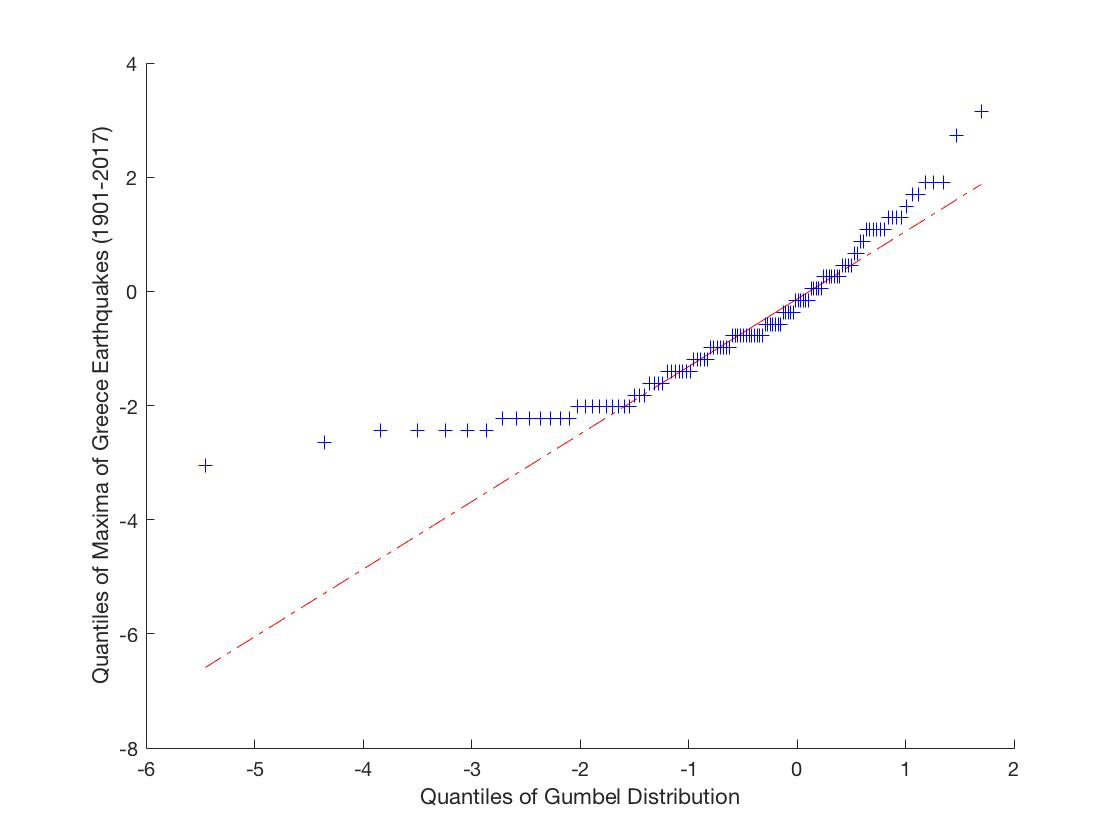
\includegraphics[width=6cm]{evmom.png}
\end{subfigure}
\begin{subfigure}
  \centering
  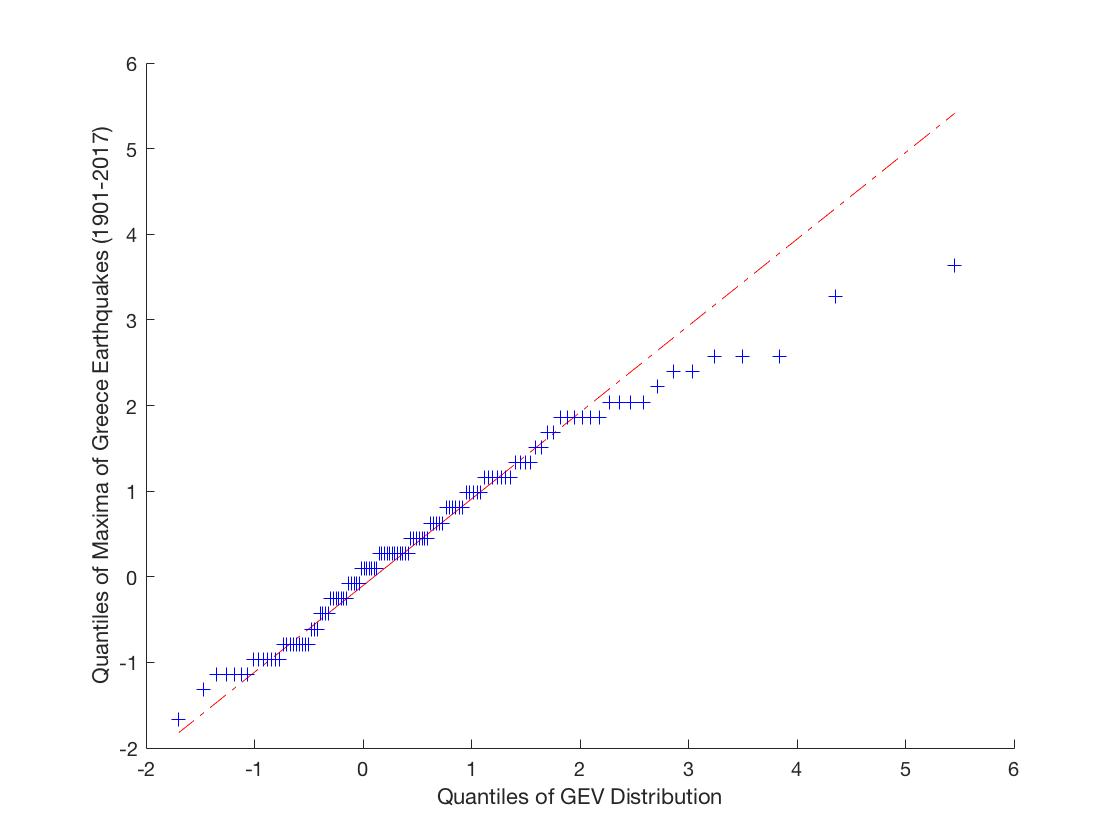
\includegraphics[width=6cm]{gevmom.png}
\end{subfigure}
  \vspace*{-5mm} 
\caption{Gumbel and GEV QQ Plots for MoM}
\centering
\begin{subfigure}
  \centering
  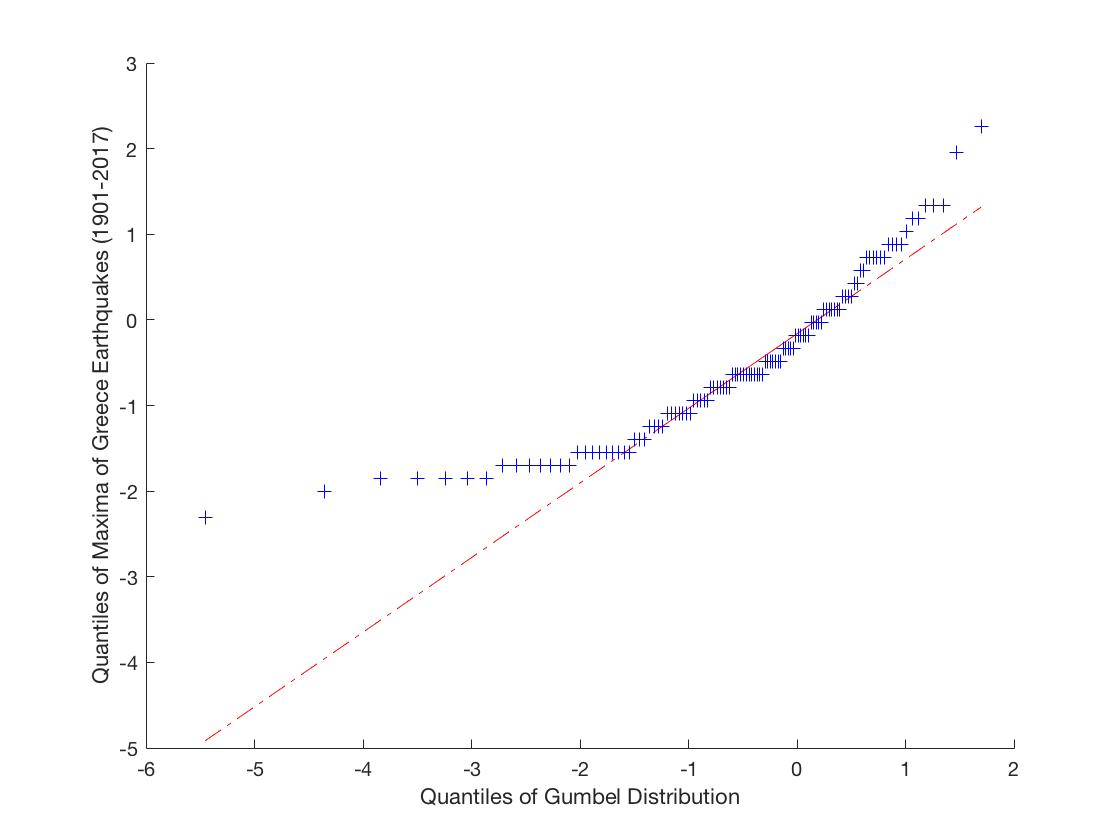
\includegraphics[width=6cm]{evmle.png}
\end{subfigure}
\begin{subfigure}
  \centering
  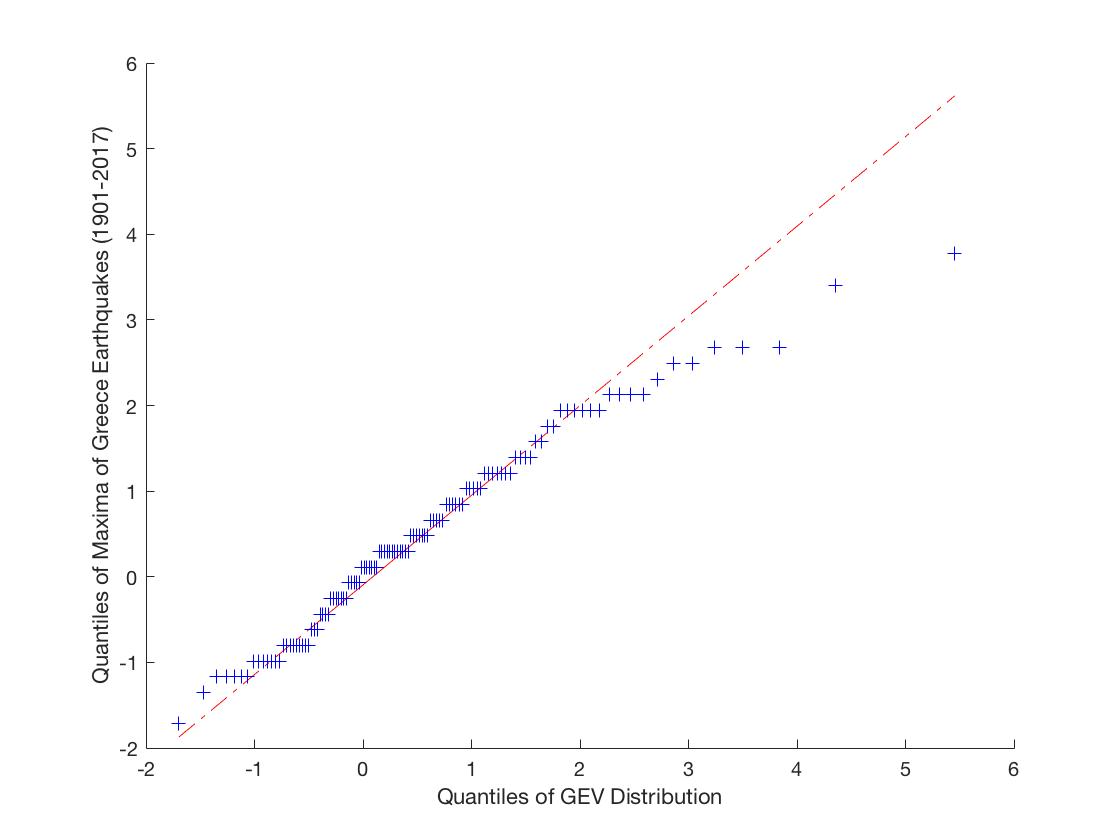
\includegraphics[width=6cm]{gevmle.png}
\end{subfigure}
  \vspace*{-5mm} 
\caption{Gumbel and GEV QQ Plots for MLE}
\centering
\begin{subfigure}
  \centering
  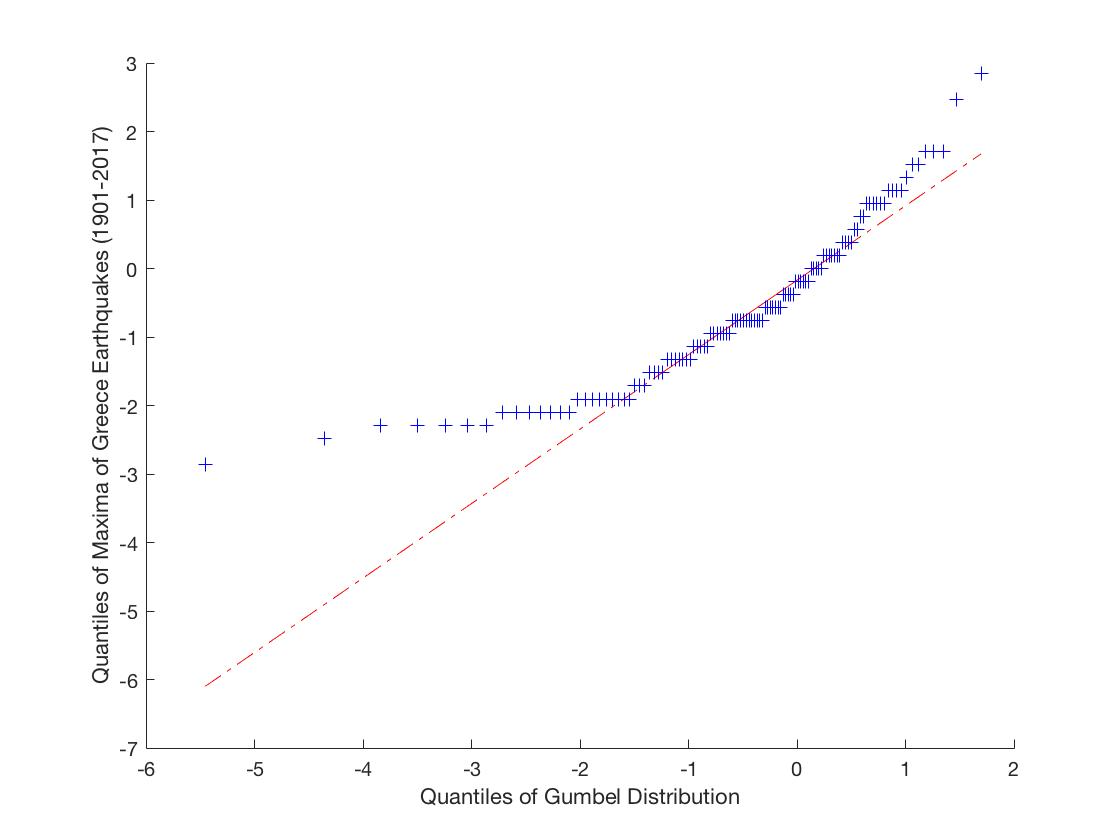
\includegraphics[width=6cm]{evpwm.png}
\end{subfigure}
\begin{subfigure}
  \centering
  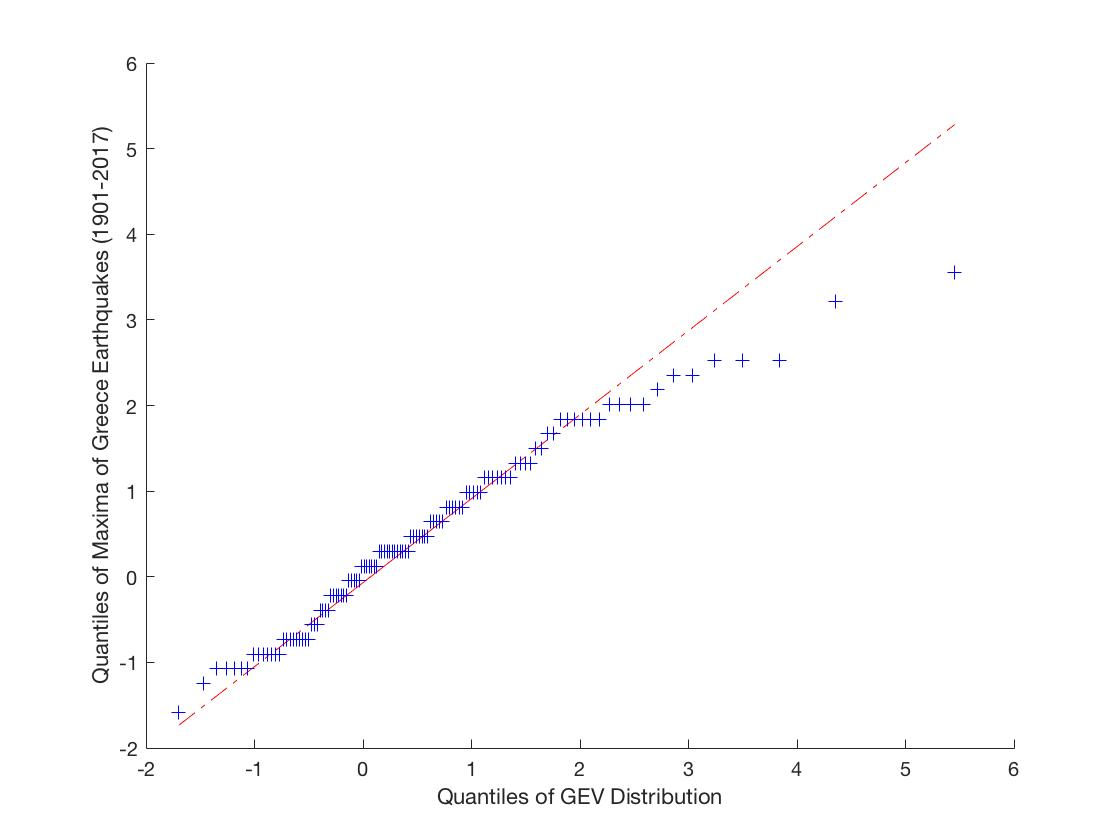
\includegraphics[width=6cm]{gevpwm.png}
\end{subfigure}
  \vspace*{-5mm}
\caption{Gumbel and GEV QQ Plots for PWM}
\end{figure}

The maxima of the Greek Earthquake data from 1901-2017 are used as the order statistics, $z_{(i)}$ so the quantiles of the input sample. The order statistics are transformed by $(z_{(i)} - \mu)/\sigma$, so that the data points would approximately fall on $y=x$ if the data follows the given distribution. The transformed order statistics are plotted against the theoretical quantiles, $y_i$ (Gumbel distribution in the first plot and GEV distribution in the second plot of each Figure).

According to the first QQ plots in Figures 9, 10 and 11 the data is skewed to the right, as the data points have a curved pattern with the slope increasing from left to right. Therefore, we can conclude the data of Greek earthquakes does not fit the Gumbel distribution when the parameters are estimated by MoM, MLE and PWM. 

In the second QQ plots in the Figures 9, 10 and 11, the data points roughly fall on $y=x$, aside from the 6 last quantiles which are taken as outliers. The QQ plots here are similar to the QQ plots of the random simulated samples of 100 from the Gumbel distribution and GEV distribution in Section 5, hence we can conclude the maxima of Greek earthquakes follows the GEV distribution. They also all have a staircase pattern, which occurs as the earthquake data is rounded to 1 decimal place.

To decide which the parameter estimations with MoM, MLE and PWM is the best, the estimation methods will be compared as the QQ plots look very similar. MLE is harder to compute in 3 parameter case, due to the iterative nature of the method, and MoM deviates with higher moments. PWM assumes $k$ between -1 and 1 but in practice $k$ is between -1/2 and 1/2. This is not an issue considering the estimated shape parameter, $k$ for Gumbel and GEV distribution, which is given in Table 1. Therefore, we can conclude PWM is a better parameter estimation method for the data of Greek Earthquakes (1901-2017). 
\newpage

\underline{\textbf{Comparison between Parameter Estimation Methods:}}

\begin{figure}[h]
\hspace*{-1cm}
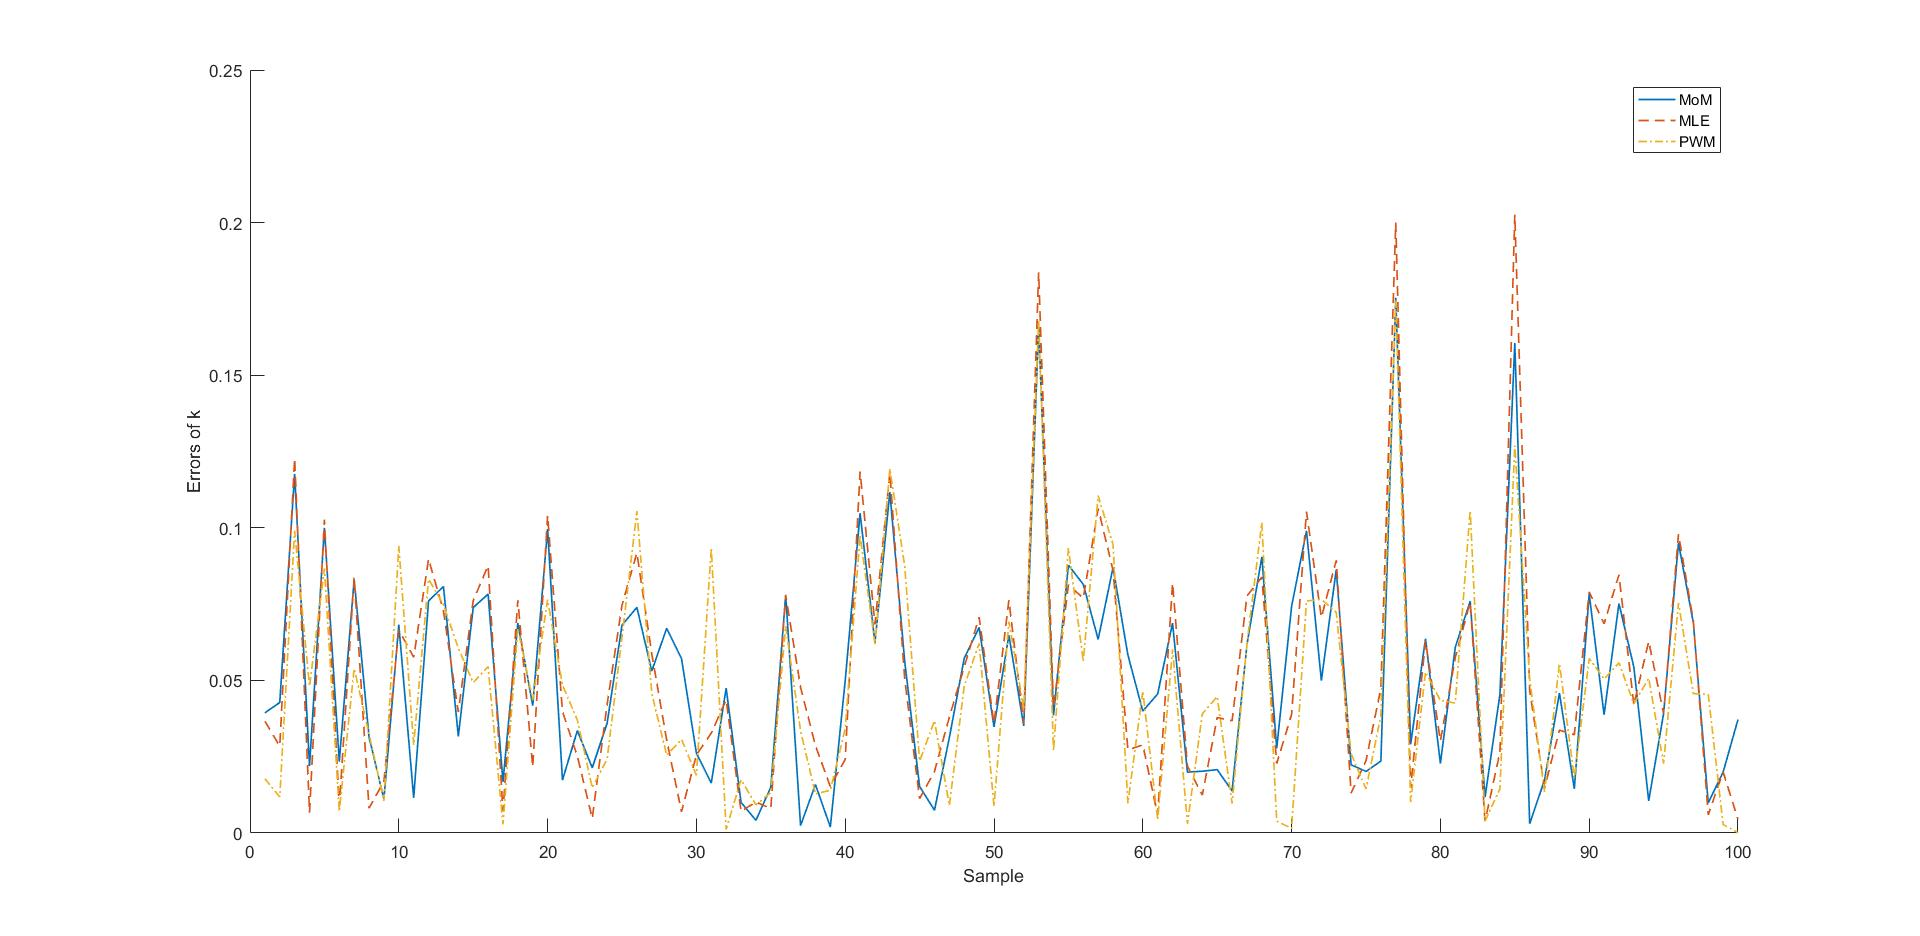
\includegraphics[width = 16.5cm, height = 10cm]{Comparison.jpg}
\vspace{-10mm}
\caption{Plot of Absolute Value of Errors of Shape Parameter}
\end{figure}

To make a further comparison among the three methods of parameter estimation, we generated 100 random sets of data with sample size, $n=117$, shape parameter, $k=-0.1$, scale parameter, $\sigma=0.56$, and location parameter, $\mu=5.94$ using the \textit{gevrnd} function in MATLAB. The estimates for $k$ using three different methods were computed and the absolute value of errors were plotted as shown in Figure 12. 

Figure 12 suggests that the errors of the estimates are pretty much the same for all three methods of estimation in most of the sets of data with the same sample size, and similar parameters as the Greek earthquakes dataset that we used. This implies that all three methods agree quite closely on the shape parameter. The mean of the errors of MoM, MLE, and PWM are 0.051, 0.053, and 0.048 respectively. The mean suggests that there is an average error of 0.05 in all three methods of estimation with PWM slightly outperforms both MoM and MLE. Hence, one would expect the true value of $k$ lies between $\pm0.05$ of the parameter estimate when estimating using these methods.
%\begin{table}[h]
%\centering
%\begin{tabular}{|c|c|c|c|} \hline
%Method: & MoM & MLE & PWM \\ \hline
%Mean: & 0.051 & 0.053 & 0.048 \\ \hline
%\end{tabular}
%\end{table}

%%%%%%%%%%%%%%%%%%%%%%%% Nishant Hypothesis Test

When studying the parameter estimates from the different methods we see a few interesting facts emerge. When trying to fit a GEV distribution we observe that the PWM and ML estimates are very close together with the shape and location parameters being the same to 2 significant figures. There is only a difference of 0.04 with the scale parameter. This suggests that for this fairly large sample ($n=117$) both the methods of probability-weighted moments and maximum likelihood perform similarly. Despite the Method of Moments being an old and simplistic method, the estimates are very similar to the PWM and ML estimates. All three estimates agree closely on the location parameter and are similar on the scale and shape parameter with the MoM estimates disagreeing with the other estimates. Nonetheless this is to be expected as, in general, the Method of Moments should only be used as an initial estimate of the parameters. All estimates agree that the shape parameter is negative which suggests that the data follows a Weibull distribution.

When fitting a Gumbel distribution to the data we see some more interesting facts. All three estimates agree quite closely on the location parameter which is higher than that of the GEV estimates. However all three estimates disagree on the scale parameter. With significant disagreement between the ML and MoM estimates. The PWM and MoM also disagree on the scale parameter for the Gumbel distribution but to a much lesser extent. However this is to be expected, as the method of Probability-Weighted Moments builds on the idea of the more simplistic and older Method of Moments.

Most importantly of all, the three estimation methods generally agree on the GEV distribution and in general disagree on the Gumbel distribution. This provides significant evidence that, in fact, the Greece earthquake data follows a GEV distribution rather than a Gumbel distribution. 

When looking at the QQ plots and estimates for our Greece earthquake data it seems to suggest that the GEV distribution seems to fit the data better than a Gumbel. Nonetheless here we perform a hypothesis test based on the PWM estimator to help verify this.

We assume that the data follows the GEV distribution with a null hypothesis that the data follows a Gumbel distribution (equivalent to assuming that the shape parameter $k=0$). We perform a 1-tailed test against the alternative hypothesis that the data follows a Weibull distribution ($k < 0$) to a 5\% significance level.

$$H_0 : k = 0, \qquad \qquad H_1 : k < 0.$$

It can be shown that the PWM estimator $\hat{k}$ is asymptotically distributed N$\left(0, 0.5633/n\right)$ (Hosking et al. 1985). For our data we have $n=117$ and the PWM estimate $\hat{k} = -0.124316$. Thus we compare the statistic
$$Z = \ddfrac{\hat{k}}{\sqrt{\frac{0.5633}{n}}} = -1.791632,$$

against the critical value $Z_c = -1.645$. Since $Z < Z_c$ we reject $H_0$ suggesting there is insufficient evidence to suggest that the data follows a Gumbel distribution to a 5\% significance level. \\

\underline{\textbf{Bootstrap Confidence Intervals:}} \\
\begin{table}[h]
\centering
\label{my-label}
\begin{tabular}{|c|c|c|c|c|c|c|}
\hline
\multirow{2}{*}{\diagbox{Parameters}{MoM}} & \multicolumn{3}{c|}{Gumbel} & \multicolumn{3}{c|}{GEV}     \\ \cline{2-7} 
                     & Estimates & CI1   & CI2   & Estimates & CI1    & CI2   \\ \hline
Location, $\mu$            & 6.478       & 6.355 & 6.603 & 5.945       & 5.827  & 6.051 \\ \hline
Scale, $\sigma$            & 0.484       & 0.430 & 0.544 & 0.566       & 0.495  & 0.639 \\ \hline
Shape, $k$              & N/A         & N/A   & N/A   & -0.147      & -0.226 & -0.049 \\ \hline
\end{tabular}
\caption{MoM Confidence Interval, [CI1, CI2] for Gumbel \& GEV }
\centering
\vspace{3mm}
\label{my-label}
\begin{tabular}{|c|c|c|c|c|c|c|}
\hline
\multirow{2}{*}{\diagbox{Parameters}{MLE}} & \multicolumn{3}{c|}{Gumbel} & \multicolumn{3}{c|}{GEV}     \\ \cline{2-7} 
                     & Estimates & CI1   & CI2   & Estimates & CI1    & CI2   \\ \hline
Location, $\mu$            & 6.519       & 6.395 & 6.645 & 5.939       & 5.808  & 6.053 \\ \hline
Scale, $\sigma$                & 0.657       & 0.578 & 0.764 & 0.547       & 0.477  & 0.621 \\ \hline
Shape, $k$              & N/A         & N/A   & N/A   & -0.122      & -0.256 & 0.036 \\ \hline
\end{tabular}
\caption{MLE Confidence Interval, [CI1, CI2] for Gumbel \& GEV }
\centering
\vspace{3mm}
\label{my-label}
\begin{tabular}{|c|c|c|c|c|c|c|}
\hline
\multirow{2}{*}{\diagbox{Parameters}{PWM}} & \multicolumn{3}{c|}{Gumbel} & \multicolumn{3}{c|}{GEV}     \\ \cline{2-7} 
                     & Estimates & CI1   & CI2   & Estimates & CI1    & CI2   \\ \hline
Location, $\mu$             & 6.503       & 6.410 & 6.675 & 5.927       & 5.803  & 6.048 \\ \hline
Scale, $\sigma$              & 0.526       & 0.514 & 0.661 & 0.583       & 0.514  & 0.661 \\ \hline
Shape, $k$               & N/A         & N/A   & N/A   & -0.124      & -0.223 & -0.012\\ \hline
\end{tabular}
\caption{PWM Confidence Interval, [CI1, CI2] for Gumbel \& GEV }
\end{table}\vspace{-0.3cm}
\\ Bootstrapping consists of resampling the maxima of Greek earthquakes (1901-2017) with replacement. To find the bootstrap confidence interval for each parameter under a certain parameter estimation method, the parameter (say $\theta$) is worked out from the initial data, $\hat{\theta}$. The data is then re-sampled 2000 times and the parameter, $\hat{\theta^{*}}$ is estimated for each sample under MoM, MLE or PWM. Then the bootstrap difference is calculated, $\delta^{*} = \hat{\theta^{*}} - \hat{\theta}$. To find the 95\% bootstrap confidence interval ($\alpha = 0.05$) of $\theta$, $\hat{\theta} - (\frac{\alpha}{2}$ quantile of $\delta^{*}$) and $\hat{\theta} -(1- \frac{\alpha}{2}$ quantile of $\delta^{*}$) are calculated, which give CI2 and CI1 respectively. This process is used to find the bootstrap confidence limits, CI1 and CI2 for a parameter (in this case $\mu$, $\sigma$ and $k$) under each parameter estimation method (MoM, MLE and PWM). 

Observing the results on Table 2, 3 and 4, none of the confidence intervals are rejected as the parameter estimates for Gumbel distribution and GEV distribution all lie in its given confidence interval, [CI1, CI2]. After incorporating the results from QQ plots, the GEV distribution (Weibull) with PWM best models the maxima of Greece Earthquakes (1901-2017).
%%%%%%%%%%%%%%%%%%%%%%%%
\vspace{-0.5cm}
\subsection{Return Period} \vspace{-0.3cm}
\begin{figure}[h]
	\centering
	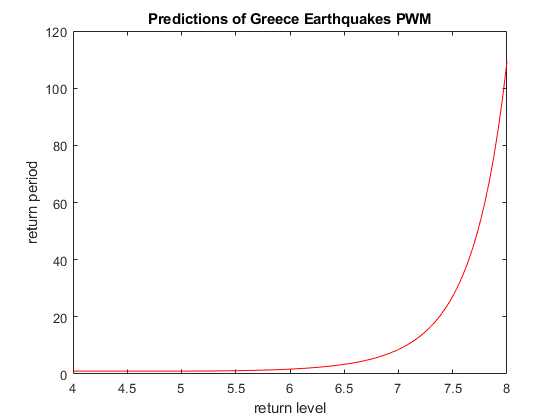
\includegraphics[width=7.5cm]{greecepwm.png}
    \vspace{-2mm}
	\caption{Predictions of Greek Earthquakes (magnitude 4.0 - 8.0)}
    \label{fig:returnperiodgreece}
\end{figure}

Figure \ref{fig:returnperiodgreece} allows us to predict how often earthquakes of magnitudes 4.0 - 8.0 will occur in Greece on average based on the dataset. We can see from Figure \ref{fig:returnperiodgreece} that on average, an earthquake of magnitude 7.5 will occur every 40 years, and an earthquake of magnitude 8 will occur every 120 years. There haven't been any earthquakes of magnitude 9 in Greece since 1901 thus we will not try to predict the average rate of those earthquakes as it would involve extrapolating from the data, rendering the prediction inaccurate. Given these predictions, we recommend that buildings in Greece be built to withstand earthquakes of magnitude 9, so that there is a minimal risk of damage when an earthquake of magnitude 8 occurs.
%%%%%%%%%%%%%%%%%%%%%%%
\newpage\vspace{-0.3cm}
\subsection{Conclusion}\vspace{-0.2cm}
In this report, the distribution of Greek earthquakes (1901-2017) was investigated using three parameter estimation methods and goodness of fit. The results suggest that Greek earthquakes follows the GEV distribution with shape parameter, $k \approx -0.12$. In terms of parameters, all three methods perform similarly when estimating $\mu$ and $\sigma$, with closer agreement in $\mu$ than in $\sigma$. On the other hand, MLE and PWM outperforms MoM when estimating $k$, suggesting that both MLE and PWM are better estimators in comparison to MoM. The comparison between estimation methods (in Figure 12) and QQ plots suggest that the estimates of PWM are slightly more accurate than MoM and MLE. Hence, by taking all these results into account, the GEV distribution with PWM gives the best fit of the maxima of Greek earthquakes.

Using this model, the return period analysis suggests that an earthquake of magnitude 8.0 will occur once every 120 years in Greece, which agrees with the data set obtained, where the largest earthquake in Greece over 117 years (1901-2017) was in 1903 with magnitude 8.0. Therefore, we conclude that the methodology used and results obtained in our study are valid and sensible, subject to minor variations dependent on the data set and field. 

The GEV distribution has played a vital role in predicting the occurrence of natural catastrophes such as earthquakes and floods over the years. The accuracy of the prediction depends highly on the estimated parameters of the model. Therefore, the process of estimating and justifying the correct parameters is essential to ensure the validity of the model and predictions obtained. 

The results in our study suggest that MoM yields unsatisfactory estimates for most of the models in comparison to MLE and PWM. This is reasonable as MoM is the simplest and oldest method for computing the estimates of a distribution. Hence, Hosking (1990) introduced the alternative approach using L-moments, defined as linear combination of order statistics, which provides more accurate estimators of parameters with small samples than MoM and MLE. (Šimková \& Picek, 2017) In the future, L-Moments should be used instead of MoM, with MLE and PWM to estimate parameters. Correct justification of the parameters is crucial to obtain a realistic seismic hazard assessment, hence the goodness of fit analysis should always be followed. 

\newpage

\section{Appendix: Code Used}

\subsection{Code for Simulated Return Plots}

\lstinputlisting{theoryreturnplot.m}

\subsection{MoM Estimation Code for Gumbel and GEV}

\textbf{\underline{MoM Estimates for Gumbel:}}

\lstinputlisting{MoMGumbel.m}

\newpage

\textbf{\underline{MoM Estimates for GEV:}}

\lstinputlisting{MoMGEV.m}

\subsection{PWM Estimation Code for Gumbel and GEV}

\textbf{\underline{PWM Estimates for Gumbel:}}

\lstinputlisting{pwmfitgumbel.m}

\textbf{\underline{PWM Estimates for GEV:}}

\lstinputlisting{pwmfitgev.m}

\subsection{Code for Bootstrap Confidence Intervals of parameters}
\textbf{\underline{Bootstrap Confidence Intervals for each parameter in the Gumbel Distribution:}}
\lstinputlisting{evpwmci.m}
(Oxenham, 2011) \\ 

\textbf{\underline{Bootstrap Confidence Interval for each parameter in the GEV Distribution:}}

\lstinputlisting{gevpwmci.m}
(Oxenham, 2011)
\newpage
\section{References}
Alves, I. \& Neves, C. (2008) \textit{Extreme Value Distribution}. Available from: \url{https://pdfs.semanticscholar.org/4c0d/a78292aa15dab79446f37b3ee73cb5c5fdec.pdf} [Accessed on 12th June 2018].

Babu, G. (2011) \textit{Model fitting, bootstrap, and model selection}. Available from: \url{http://astrostatistics.psu.edu/RLectures/model\_selection\_gof-bootstrap.pdf} 
[Accessed on 8th June 2018].

Bhunya, P. K., Jain, S. K., Ojha, C. S. \& Agarwal, A. (2007) Simple parameter 
estimation technique for three-parameter generalized extreme value distribution. 
\textit{Journal of hydrologic engineering}. 12(6), 682-689. Available from: DOI:  
10.1061/(ASCE)1084-0699(2007)12:6(682). 

Castillo, E. (1988) \textit{Extreme Value Theory in Engineering}. Academic Press, inc.(London) LTD.

Coles, S. (2001) \textit{An introduction to statistical modeling of extreme values.} Springer.

Geyer, C. (2012) \textit{Lecture Slides Deck 8.} [Presentation] Stat 5102. University of Minnesota, 12th March. Available from: \url{http://www.stat.umn.edu/geyer/s12/5102/slides/s8.pdf} [Accessed on 8th June 2018].

Greenwood, J. A., Landwehr, J. M., Matalas, N. C. \& Wallis, J. R. (1979) Probability 
weighted moments: definition and relation to parameters of several distributions 
expressable in inverse form. \textit{Water resources research}. 15(5), 1049-1054. 
Available from: DOI: 10.1029/WR015i005p01049. 

Haan, L. \& Ferreira, A. (2006). \textit{Extreme Value Theory, An Introduction}. Springer, New York.

%Hallsworth, C. (2017) \textit{The method of moments}. [Lecture] Probability and 
%Statistics II (M2S1). Imperial College London, 24th November.

Hosking, J. R. M. (1990) L-moments: Analysis and estimation of distributions using linear combinations of order statistics. \textit{Journal of the Royal Statistical Society, Series B.} 52(1), 105–124. Available from: DOI: 10.2307/2345653.

Hosking, J. R. M., Wallis, J. R. \& Wood, E. F. (1985) Estimation of the generalized 
extreme value distribution by the method of probability-weighted moments. 
\textit{Technometrics}. 27(3), 251-261. Available from: DOI: 10.2307/1269706.

Institute of Geodynamics, National Observatory of Athens. (2018) \textit{Earthquakes catalogues.} Available from: \url{http://www.gein.noa.gr/en/seismicity/earthquake-catalogs} [Accessed on 13th June 2018].

Jost, S. (2018) \textit{Normal Plots.} Available from: \url{http://condor.depaul.edu/sjost/it223/documents/normal-plot.htm} [Accessed on 5th June 2018]. 

Kotz, S. \& Nadarajah, S. (2000) \textit{Extreme value distributions: theory and 
applications.} Imperial College Press. 

Mahdi, S. \& Cenac, M. (2004) Estimating parameters of Gumbel distribution using the 
methods of moments, probability weighted moments and maximum likelihood. \textit{Revista
de Matemática: Teoría y Aplicaciones}. 12(1-2), 151-156. Available from: DOI: 10.15517/rmta.v12i1-2.259.

MathWorks. (2018) \textit{QQ Plot.} Available from:
\url{https://uk.mathworks.com/help/stats/qqplot.html} [Accessed on 11th June 2018].

MathWorks. (2018a) \textit{evfit}. Available from: \url{https://uk.mathworks.com/help/stats/evfit.html}[Accessed on 17th June 2018].

MathWorks. (2018b) \textit{gevfit}. Available form: \url{https://uk.mathworks.com/help/stats/gevfit.html}[Accessed on 17th June 2018].

Nadarajah, S. (2018a) \textit{The extremal types theorem.} Available from: \url{http://www.maths.manchester.ac.uk/~saralees/ettproof.pdf} [Accessed on 16th June 2018].

Nadarajah, S. (2018b) \textit{Fundamental of extreme value theory.} Available from: \url{http://www.maths.manchester.ac.uk/~saralees/chap1.pdf} [Accessed on 16th June 2018].

National Aeronautics and Space Administration. (2018) \textit{Generalized extreme value distribution and calculation of return value.} Available from: \url{https://gmao.gsfc.nasa.gov/research/subseasonal/atlas/GEV-RV-html/GEV-RV-description.html}[Accessed on 9th June 2018].

Orloff, J. \& Bloom, J. (2014) \textit{Bootstrap confidence intervals.} 
Available from: \url{https://ocw.mit.edu/courses/mathematics/18-05-introduction-to-probability-and-statistics-spring-2014/readings/MIT18_05S14_Reading24.pdf} [Accessed on 8th June 2018].

Oxenham. A. (2011) \textit{Lesson 6: Introduction to the Bootstrap.} Available from:
\url{http://www.mbfys.ru.nl/~robvdw/DGCN22/PRACTICUM_2011/LABS_2011/ALTERNATIVE_LABS/Lesson_6.html} [Accessed on 13rd June 2018].

Rasmussen, P. F. \& Gautam, N. (2003) Alternative PWM-estimators of the Gumbel distribution. \textit{Journal of Hydrology}. 280(1-4), 265-271. Available from: DOI: 10.1016/S0022-1694(03)00241-5.

Scott, D. (2018) \textit{Quantile-Quantile (q-q) plots.} Available from: \url{http://onlinestatbook.com/2/advanced_graphs/q-q_plots.html} [Accessed on 1st June 2018].

Šimková, T. \& Picek, J. (2017) A comparison of L-, LQ-, TL-moment and
maximum likelihood high quantile estimates of the GPD and GEV distribution. \textit{Communications in statistics - Simulation and computation}. 46(8), 5991-6010, Available from: 10.1080/03610918.2016.1188206

Smith, R. (2009) \textit{Extreme value theory.} Available from: \url{https://www.unc.edu/~rls/s890/evtclass.pdf} [Accessed on 2nd June 2018].

Stedinger, J. R. \& Martins, E. S. (2000). \textit{Generalized maximum-likelihood generalized extreme-value
quantile estimators for hydrologic data}. Available from: \url{http://citeseerx.ist.psu.edu/viewdoc/download?doi=10.1.1.463.9611&rep=rep1&type=pdf}[Accessed 16th June 2018].

Stedinger, J. R., Vogel, R. M., \& Foufoula-Georgiou, E. (1993) Frequency analysis of extreme events. \textit{Handbook of hydrology}. 18. Available from: \url{https://engineering.tufts.edu/cee/people/vogel/documents/frequencyAnalysis.pdf} [Accessed 14th June 2018].

Stefopoulos, A. (2018) \textit{Earthquakes in Greece (1901-2018).} Available from: \url{https://www.kaggle.com/astefopoulos/earthquakes-in-greece-19012018} [Accessed 13th June 2018].

Sun, R. (2018) \textit{Lecture 12}. Available from: \url{http://www.math.nus.edu.sg/~matsr/ProbI/Lecture12.pdf}[Accessed 15th June 2018].

U.S. Geological Survey. (2018) \textit{Why are we having so many earthquakes?.} Available from: \url{https://tinyurl.com/ya726dwd} [Accessed on 17 June 2018]. (The link has been compressed using \url{http://tinyurl.com})

Wilk, M. B. \& Gnanadesikan R. (1968) Probability plotting methods for the analysis of data. \textit{Biometrika}. 55(1), 1-17. Available from: DOI: 10.2307/2334448.


\end{document}